%
% chapter.tex -- Spezielle Funktionen definiert durch Integrale
%
% (c) 2021 Prof Dr Andreas Müller, Hochschule Rapperswil
%
% !TeX spellcheck = de_CH
\chapter{Orthogonalität
\label{buch:chapter:orthogonalitaet}}
\lhead{Orthogonalität}
\rhead{}
In der linearen Algebra lernt man, dass orthonormierte Basen für die
Lösung vektorgeometrischer Probleme, bei denen auch das Skalarprodukt
involviert ist, besonders günstig sind.
Die Zerlegung eines Vektors in einer Basis verlangt normalerweise nach
der Lösung eines linearen Gleichungssystems, für orthonormierte
Basisvektoren beschränkt sie sich auf die Berechnung von Skalarprodukten.

Oft dienen spezielle Funktionen als Basis der Lösungen einer linearen
partiellen Differentialgleichung (siehe Kapitel~\ref{buch:chapter:pde}).
Die Randbedingungen müssen dazu in der gewählten Basis von Funktionen
zerlegt werden.
Fourier ist es gelungen, die Idee des Skalarproduktes und der Orthogonalität
auf Funktionen zu verallgemeinern und so zum Beispiel das Wärmeleitungsproblem
zu lösen.

Der Orthonormalisierungsprozess von Gram-Schmidt wird damit auch auf
Funktionen anwendbar
(Abschnitt~\ref{buch:orthogonalitaet:section:orthogonale-funktionen}),
der Nutzen führt aber noch viel weiter.
Da $K[x]$ ein Vektorraum ist, führt er von der Basis der Monome
$\{1,x,x^2,\dots,x^n\}$ 
auf orthonormierte Polynome.
Diese haben jedoch eine ganze Reihe weiterer nützlicher Eigenschaften.
So wird in Abschnitt~\ref{buch:orthogonal:section:drei-term-rekursion}
gezeigt, dass sich die Werte aller Polynome einer solchen Familie mit
einer Rekursionsformel effizient berechnen lassen, die höchstens drei
Terme umfasst.
In Abschnitt~\ref{buch:orthogonalitaet:section:rodrigues} werden
die Rodrigues-Formeln vorgeführt, die Polynome durch Anwendung eines
Differentialoperators hervorbringen.
In Abschnitt~\ref{buch:orthogonal:section:orthogonale-polynome-und-dgl}
schliesslich wird gezeigt, dass diese Polynome auch Eigenfunktionen
eines selbstadjungierten Operators sind.
Da man in der linearen Algebra auch lernt, dass die Eigenvektoren einer
symmetrischen Matrix zu verschiedenen Eigenwerten orthogonal sind,
ist die Orthogonalität plötzlich nicht mehr überraschend.

Die Bessel-Funktionen von
Abschnitt~\ref{buch:differntialgleichungen:section:bessel}
sind auch Eigenfunktionen eines Differentialoperators.
Abschnitt~\ref{buch:orthogonalitaet:section:bessel} findet das zugehörige
Skalarprodukt, welches andeutet, dass auch für andere Funktionenfamilien
eine entsprechende Konstruktion möglich ist.
Das in Abschnitt~\ref{buch:integrale:subsection:sturm-liouville-problem}
präsentierte Sturm-Liouville-Problem führt sie durch.
Das Kapitel schliesst mit dem
Abschnitt~\ref{buch:orthogonal:section:gauss-quadratur}
über die Gauss-Quadratur, welche die Eigenschaften orthogonaler Polynome
für einen besonders effizienten numerischen Integrationsalgorithmus
ausnutzt.

%
% orthogonal.tex
%
% (c) 2021 Prof Dr Andreas Müller, OST Ostschweizer Fachhochschule
%
\section{Orthogonalität
\label{buch:integral:section:orthogonale-polynome}}
\rhead{Orthogonale Polynome}
Die Fourier-Theorie basiert auf der Idee, Funktionen durch 
Funktionenreihen mit Summanden zu bilden, die im Sinne eines
Skalarproduktes orthogonal sind, welches mit Hilfe eines Integrals
definiert sind.
Solche Funktionenfamilien treten jedoch auch als Lösungen von
Differentialgleichungen.
Besonders interessant wird die Situation, wenn die Funktionen 
Polynome sind.

%
% Skalarprodukt
%
\subsection{Skalarprodukt}
Der reelle Vektorraum $\mathbb{R}^n$ trägt das Skalarprodukt
\[
\langle\;\,,\;\rangle
\colon
\mathbb{R}^n \times \mathbb{R}^n \to \mathbb{R}
:
(x,y)\mapsto \langle x, y\rangle = \sum_{k=1}^n x_iy_k,
\]
welches viele interessante Anwendungen ermöglicht.
Eine orthonormierte Basis macht es zum Beispiel besonders leicht,
eine Zerlegung eines Vektors in dieser Basis zu finden.
In diesem Abschnitt soll zunächst an die Eigenschaften erinnert
werden, die zu einem nützlichen 

\subsubsection{Eigenschaften eines Skalarproduktes}
Das Skalarprodukt erlaubt auch, die Länge eines Vektors $v$
als $|v| = \sqrt{\langle v,v\rangle}$ zu definieren.
Dies funktioniert natürlich nur, wenn die Wurzel auch immer
definiert ist, d.~h.~das Skalarprodukt eines Vektors mit sich
selbst darf nicht negativ sein.
Dazu dient die folgende Definition.

\begin{definition}
Sei $V$ ein reeller Vektorraum.
Eine bilineare Abbildung
\[
\langle\;\,,\;\rangle
\colon
V\times V
\to
\mathbb{R}
:
(u,v) \mapsto \langle u,v\rangle.
\]
heisst {\em positiv definit}, wenn für alle Vektoren $v \in V$ mit
$v\ne 0 \Rightarrow \langle v,v\rangle > 0$ 
Die {\em Norm} eines Vektors $v$ ist
$|v|=\sqrt{\langle v,v\rangle}$.
\end{definition}

Damit man mit dem Skalarprodukt sinnvoll rechnen kann, ist ausserdem
erforderlich, dass es eine einfache Beziehung zwischen 
$\langle x,y\rangle$ und $\langle y,x\rangle$ gibt.

\begin{definition}
Ein {\em Skalarprodukt} auf einem reellen Vektorraum $V$ ist eine
positiv definite, symmetrische bilineare Abbildung
\[
\langle\;\,,\;\rangle
\colon
V\times V
\to
\mathbb{R}
:
(u,v) \mapsto \langle u,v\rangle.
\]
\end{definition}

Das Skalarprodukt $\langle u,v\rangle=u^tv$ auf dem Vektorraum 
$\mathbb{R}^n$ erfüllt die Definition ganz offensichtlich,
sie führt auf die Komponentendarstellung
\[
\langle u,v\rangle = u^tv = \sum_{k=1}^n u_iv_i.
\]
Weitere Skalarprodukte ergeben ergeben sich mit jeder symmetrischen,
positiv definiten Matrix $G$ und der Definition
$\langle u,v\rangle_G=u^tGv$.
Ein einfacher Spezialfall tritt auf, wenn $G$ eine Diagonalmatrix
$\operatorname{diag}(w_1,\dots,w_n)$
mit positiven Einträgen $w_i>0$ auf der Diagonalen ist.
In diesem Fall schreiben wir
\[
\langle u,v\rangle_w
=
u^t\operatorname{diag}(w_1,\dots,w_n)v
=
\sum_{k=1}^n u_iv_i\,w_i
\]
und nennen $\langle \;\,,\;\rangle_w$ das {\em gewichtete Skalarprodukt}
mit {\em Gewichten $w_i$}.

\subsubsection{Skalarprodukte auf Funktionenräumen}
Das Integral ermöglicht jetzt, ein Skalarprodukt auf dem reellen
Vektorraum der stetigen Funktionen auf einem Intervall zu definieren.

\begin{definition}
Sei $V$ der reelle Vektorraum $C([a,b])$ der reellwertigen, stetigen
Funktion auf dem Intervall $[a,b]$.
Dann ist 
\[
\langle\;\,,\;\rangle
\colon
C([a,b]) \times C([a,b]) \to \mathbb{R}
:
(f,g) \mapsto \langle f,g\rangle = \int_a^b f(x)g(x)\,dx.
\]
ein Skalarprodukt.
\end{definition}

Die Definition ist offensichtlich symmetrisch in $f$ und $g$ und
aus den Eigenschaften des Integrals ist klar, dass das Produkt
bilinear ist:
\begin{align*}
\langle \lambda_1 f_1+\lambda_2f_2,g\rangle
&=
\int_a^b (\lambda_1f_(x) +\lambda_2f_2(x))g(x)\,dx
=
\lambda_1\int_a^b f_1(x) g(x)\,dx
+
\lambda_2\int_a^b f_2(x) g(x)\,dx
\\
&=
\lambda_1\langle f_1,g\rangle
+
\lambda_2\langle f_2,g\rangle.
\end{align*}
Ausserdem ist es positiv definit, denn wenn $f(x_0) \ne 0$ ist,
dann gibt es wegen der Stetigkeit von $f$ eine Umgebung
$U=[x_0-\varepsilon,x_0+\varepsilon]$, derart, dass $|f(x)| > \frac12|f(x_0)|$
ist für alle $x\in U$.
Somit ist das Integral
\[
\langle f,f\rangle
=
\int_a^b |f(x)|^2\,dx
\ge
\int_{x_0-\varepsilon}^{x_0+\varepsilon} |f(x)|^2\,dx
\ge
\int_{x_0-\varepsilon}^{x_0+\varepsilon} \frac14|f(x_0)|^2\,dx
=
\frac{1}{4}|f(x_0)|^2\cdot 2\varepsilon
=
\frac{|f(x_0)|\varepsilon}{2}
>0,
\]
was beweist, dass $\langle\;,\;\rangle$ positiv definit und damit
ein Skalarprodukt ist.

Die Definition kann noch etwas verallgemeinert werden, indem 
die Funktionswerte nicht überall auf dem Definitionsbereich 
gleich gewichtet werden. 

\begin{definition}
Sei $w\colon [a,b]\to \mathbb{R}^+$ eine positive, stetige Funktion,
dann ist
\[
\langle\;\,,\;\rangle_w
\colon
C([a,b]) \times C([a,b]) \to \mathbb{R}
:
(f,g) \mapsto \langle f,g\rangle_w = \int_a^b f(x)g(x)\,w(x)\,dx.
\]
das {\em gewichtete Skalarprodukt} mit {\em Gewichtsfunktion $w(x)$}.
\end{definition}

\subsubsection{Gram-Schmidt-Orthonormalisierung}
In einem reellen Vektorraum $V$ mit Skalarprodukt $\langle\;\,,\;\rangle$
kann aus einer beleibigen Basis $b_1,\dots,b_n$ mit Hilfe des 
Gram-Schmidtschen Orthogonalisierungsverfahrens immer eine
orthonormierte Basis $\tilde{b}_1,\dots,\tilde{b}_n$ Basis
gewonnen werden.
Es stellt sicher, dass für alle $k\le n$ gilt
\[
\langle b_1,\dots,b_k\rangle
=
\langle \tilde{b}_1,\dots,\tilde{b}_k\rangle.
\]
Zur Vereinfachung der Formeln schreiben wir $v^0=v/|v|$ für einen zu
$v$ parallelen Einheitsvektor.
Die Vektoren $\tilde{b}_i$ können mit Hilfe der Formeln
\begin{align*}
\tilde{b}_1
&=
(b_1)^0
\\
\tilde{b}_2
&=
\bigl(
b_2
-
\langle \tilde{b}_1,b_2\rangle \tilde{b}_1
\bigr)^0
\\
\tilde{b}_3
&=
\bigl(
b_3
-
\langle \tilde{b}_1,b_3\rangle \tilde{b}_1
-
\langle \tilde{b}_2,b_3\rangle \tilde{b}_2
\bigr)^0
\\
&\;\vdots
\\
\tilde{b}_n
&=
\bigl(
b_n
-
\langle \tilde{b}_1,b_n\rangle \tilde{b}_1
-
\langle \tilde{b}_2,b_n\rangle \tilde{b}_2
-\dots
-
\langle \tilde{b}_{n-1},b_n\rangle \tilde{b}_{n-1}
\bigr)^0
\end{align*}
iterativ berechnet werden.
Dieses Verfahren lässt sich auch auf Funktionenräume anwenden.

Die Normierung ist nicht unbedingt nötig und manchmal unangenehm,
da die Norm unschöne Quadratwurzeln einführt.
Falls es genügt, eine orthogonale Basis zu finden, kann darauf
verzichtet werden, bei der Orthogonalisierung muss aber berücksichtigt
werden, dass die Vektoren $\tilde{b}_i$ jetzt nicht mehr Einheitslänge
haben.
Die Formeln
\begin{align*}
\tilde{b}_0
&=
b_0
\\
\tilde{b}_1
&=
b_1
-
\frac{\langle b_1,\tilde{b}_0\rangle}{\langle \tilde{b}_0,\tilde{b}_0\rangle}\tilde{b}_0
\\
\tilde{b}_2
&=
b_2
-
\frac{\langle b_2,\tilde{b}_0\rangle}{\langle \tilde{b}_0,\tilde{b}_0\rangle}\tilde{b}_0
-
\frac{\langle b_2,\tilde{b}_1\rangle}{\langle \tilde{b}_1,\tilde{b}_1\rangle}\tilde{b}_1
\\
&\;\vdots
\\
\tilde{b}_n
&=
b_n
-
\frac{\langle b_n,\tilde{b}_0\rangle}{\langle \tilde{b}_0,\tilde{b}_0\rangle}\tilde{b}_0
-
\frac{\langle b_n,\tilde{b}_1\rangle}{\langle \tilde{b}_1,\tilde{b}_1\rangle}\tilde{b}_1
-
\dots
-
\frac{\langle b_n,\tilde{b}_{n-1}\rangle}{\langle \tilde{b}_{n-1},\tilde{b}_{n-1}\rangle}\tilde{b}_{n-1}.
\end{align*}
berücksichtigen dies.


%
% Orthogonale Polynome
%
\subsection{Orthogonale Polynome
\label{buch:integral:subsection:orthogonale-polynome}}
Die Polynome $1,x,x^2,\dots,x^n$ bilden eine Basis des Vektorraums
der Polynome vom Grad $\le n$.
Bezüglich des Skalarproduktes
\[
\langle p,q\rangle
=
\int_{-1}^1 p(x)q(x)\,dx
\]
sind sie jedoch nicht orthogonal, denn es ist
\[
\langle x^i,x^j\rangle
=
\int_{-1}^1 x^{i+j}\,dx
=
\biggl[\frac{x^{i+j+1}}{i+j+1}\biggr]_{-1}^1
=
\begin{cases}
\displaystyle
\frac{2}{i+j+1}&\qquad\text{$i+j$ gerade}\\
              0&\qquad\text{$i+j$ ungerade}.
\end{cases}
\]
Wir können daher das Gram-Schmidtsche Orthonormalisierungsverfahren
anwenden, um eine orthogonale Basis von Polynomen zu finden, was
wir im Folgenden tun wollen.

% XXX Orthogonalisierungsproblem so formulieren, dass klar wird,
% XXX dass man ein "Normierungskriterium braucht.

Da wir auf die Normierung verzichten, brauchen wir ein anderes
Kriterium, welches die Polynome eindeutig festlegen kann.
Wir bezeichnen das Polynom vom Grad $n$, das bei diesem Prozess
entsteht, mit $P_n(x)$ und legen willkürlich aber traditionskonform
fest, dass $P_n(1)=1$ sein soll.

Das Skalarprodukt berechnet ein Integral eines Produktes von zwei
Polynomen über das symmetrische Interval $[-1,1]$.
Ist die eine gerade und die andere ungerade, dann ist das
Produkt eine ungerade Funktion und das Skalarprodukt verschwindet.
Sind beide Funktionen gerade oder ungerade, dann ist das Produkt
gerade und das Skalarprodukt ist im Allgmeinen von $0$ verschieden.
Dies zeigt, dass es tatsächlich etwas zu Orthogonalisieren gibt.

Die ersten beiden Funktionen sind das konstante Polynom $1$ und
das Polynome $x$.
Nach obiger Beobachtung ist das Skalarprodukt $\langle 1,x\rangle=0$,
also ist $P_1(x)=x$.

\begin{lemma}
Die Polynome $P_{2n}(x)$ sind gerade, die Polynome $P_{2n+1}(x)$ sind
ungerade Funktionen von $x$.
\end{lemma}

\begin{proof}[Beweis]
Wir verwenden vollständige Induktion nach $n$.
Wir wissen bereits, dass $P_0(x)=1$ und $P_1(x)=x$ die verlangten
Symmetrieeigenschaften haben.
Im Sinne der Induktionsannahme nehmen wir daher an, dass die
Symmetrieeigenschaften für $P_k(x)$, $k<n$, bereits bewiesen sind.
$P_n(x)$ entsteht jetzt durch Orthogonalisierung nach der Formel
\[
P_n(x)
=
x^n
-
\langle P_{n-1},x^n\rangle P_{n-1}(x)
-
\langle P_{n-2},x^n\rangle P_{n-2}(x)
-\dots-
\langle P_1,x^n\rangle P_1(x)
-
\langle P_0,x^n\rangle P_0(x).
\]
Die Skalarprodukte
$\langle P_{n-1},x^n\rangle$,
$\langle P_{n-3},x^n\rangle$, $\dots$ verschwinden alle, so dass
$P_n(x)$ eine Linearkombination der Funktionen $x^n$, $P_{n-2}(x)$,
$P_{n-4}(x)$ ist, die die gleiche Parität wie $x^n$ haben.
Also hat auch $P_n(x)$ die gleiche Parität, was das Lemma beweist.
\end{proof}

Die Ortogonalisierung von $x^2$ liefert daher
\[
p(x) = x^2
-
\frac{\langle x^2,P_0\rangle}{\langle P_0,P_0\rangle} P_0(x)
=
x^2 - \frac{\int_{-1}^1x^2\,dx}{\int_{-1}^11\,dx}
=
x^2 - \frac{\frac{2}{3}}{2}=x^2-\frac13
\]
Dieses Polynom erfüllt die Standardisierungsbedingung noch 
nicht den $p(1)=\frac23$.
Daraus leiten wir ab, dass
\[
P_2(x) = \frac12(3x^2-1)
\]
ist.

Für $P_3(x)$ brauchen wir nur die Skalaprodukte
\[
\left.
\begin{aligned}
\langle x^3,P_1\rangle
&=
\int_{-1}^1  x^3\cdot x\,dx
=
\biggl[\frac15x^5\biggr]_{-1}^1
=
\frac25
\qquad
\\
\langle P_1,P_1\rangle
&=
\int_{-1}^1 x^2\,dx
=
\frac23
\end{aligned}
\right\}
\qquad
\Rightarrow
\qquad
p(x) = x^3 - \frac{\frac25}{\frac23}x=x^3-\frac{3}{5}x
\]
Die richtige Standardisierung ergibt sich,
indem man durch $p(1)=\frac25$ dividiert, also
\[
P_2(x) = \frac12(5x^3-3x).
\]

Die Berechnung weiterer Polynome verlangt, dass Skalarprodukte
$\langle x^n,P_k\rangle$ berechnet werden müssen, was wegen
der zunehmend komplizierten Form von $P_k$ etwas mühsam ist.
Wir berechnen den Fall $P_4$.
Dazu muss das Polynom $x^4$ um eine Linearkombination von
$P_2$ und $P_0(x)=1$ korrigiert werden.
Die Skalarprodukte sind
\begin{align*}
\langle x^4, P_0\rangle
&=
\int_{-1}^1 x^4\,dx = \frac25
\\
\langle P_0,P_0\rangle
&=
\int_{-1}^1 \,dx = 2
\\
\langle x^4,P_2\rangle
&=
\int_{-1}^1 \frac32x^6-\frac12 x^4\,dx
=
\biggl[\frac{3}{14}x^7-\frac{1}{10}x^5\biggr]_{-1}^1
=
\frac6{14}-\frac15
=
\frac8{35}
\\
\langle P_2,P_2\rangle
&=
\int_{-1}^1 \frac14(3x^2-1)^2\,dx
=
\int_{-1}^1 \frac14(9x^4-6x^2+1)\,dx
=
\frac14(\frac{18}{5}-4+2)
=\frac25.
\end{align*}
Daraus folgt für $p(x)$
\begin{align*}
p(x)
&=
x^4
-
\frac{\langle x^4,P_2\rangle}{\langle P_2,P_2\rangle}P_2(x)
-
\frac{\langle x^4,P_0\rangle}{\langle P_0,P_0\rangle}P_0(x)
\\
&=
x^4
-\frac47 P_2(x) - \frac15 P_0(x)
\\
&=
x^4 - \frac{6}{7}x^2 + \frac{3}{35}
\end{align*}
mit $p(1)=\frac{8}{35}$, so dass man
\[
P_4(x) =
\frac18(35x^4-30x^2+3)
\]
setzen muss.

\begin{table}
\centering
\renewcommand{\arraystretch}{1.5}
\begin{tabular}{|>{$}c<{$}|>{$}l<{$}|}
\hline
n&P_n(x)\\
\hline
 0&1
\\
 1&x
\\
 2&\frac12(3x^2-1)
\\
 3&\frac12(5x^3-3x)
\\
 4&\frac18(35x^4-30x^2+3)
\\
 5&\frac18(63x^5-70x^3+15x)
\\
 6&\frac1{16}(231x^6-315x^4+105x^2-5)
\\
 7&\frac1{16}(429x^7-693x^5+315x^3-35x)
\\
 8&\frac1{128}(6435x^8-12012x^6+6930x^4-1260x^2+35)
\\
 9&\frac1{128}(12155x^9-25740x^7+18018x^5-4620x^3+315x)
\\
10&\frac1{256}(46189x^{10}-109395x^8+90090x^6-30030x^4+3465x^2-63)
\\
\hline
\end{tabular}
\caption{Die Legendre-Polynome $P_n(x)$ für $n=0,1,\dots,10$ sind
orthogonale Polynome vom Grad $n$, die den Wert $P_n(1)=1$ haben.
\label{buch:integral:table:legendre-polynome}}
\end{table}

Die so konstruierten Polynome heissen die {\em Legendre-Polynome}.
Durch weitere Durchführung des Verfahrens liefert die Polynome in
Tabelle~\ref{buch:integral:table:legendre-polynome}.


%%
%% Differentialgleichungen
%%
%\subsection{Orthogonale Polynome und Differentialgleichungen}
%\subsubsection{Legendre-Differentialgleichung}
%\subsubsection{Legendre-Polyome}
%\subsubsection{Legendre-Funktionen zweiter Art}
%Siehe Wikipedia-Artikel \url{https://de.wikipedia.org/wiki/Legendre-Polynom}

%
% legendredgl.tex
%
% (c) 2021 Prof Dr Andreas Müller, OST Ostschweizer Fachhochschule
%
\subsection{Orthogonale Polynome und Differentialgleichungen}
Legendre hat einen ganz anderen Zugang zu den nach ihm benannten
Polynomen gefunden.
Er hat sie gefunden als die Lösungen einer speziellen Differentialgleichungen.
In diesem Abschnitt sollen diese Funktionen mit der Potenzreihen-Methode
wiedergefunden werden.
Dabei stellt sich heraus, dass diese Polynome auch Eigenfunktionen eines
selbstadjungierten Differentialgoperator sind.
Die Orthogonalität wird dann aus einer Verallgemeinerung der bekannten
Eingeschaft folgen, dass Eigenvektoren einer symmetrischen Matrix zu 
verschiedenen Eigenwerten orthogonal sind.

\subsubsection{Legendre-Differentialgleichung}
Die {\em Legendre-Differentialgleichung} ist die Differentialgleichung
\begin{equation}
(1-x^2) y'' - 2x y' + n(n+1) y = 0
\label{buch:integral:eqn:legendre-differentialgleichung}
\end{equation}
für eine Funktion $y(x)$ auf dem Intervall $[-1,1]$.

Sei $y(x)$ eine Lösung der Differentialgleichung
\eqref{buch:integral:eqn:legendre-differentialgleichung}.
Setzt man $y_s(x)=y(-x)$ in die Differentialgleichung ein, erhält
man
\[
(1-x^2)y_s''(x) - 2x y'_s(x) + n(n+1)y_s(x)
=
(1-x^2)y''(-x) +2x y(-x) +n(n+1)y(-x).
\]
Ersetzt man $t=-x$, dann wird daraus
\[
(1-x^2)y''(t) -2t y(t) + n(n+1) y(t) = 0
\]
aus der Differentialgleichung
\eqref{buch:integral:eqn:legendre-differentialgleichung}.
Insbesondere ist die gespiegelte Funktion $y_s(x)$ ebenfalls
eine Lösung der Differentialgleichung.

Ist $y(x)$ eine Lösung der Differentialgleichung ist, dann lässt
sie sich in die Summe einer geraden und einer ungeraden Funktion
\[
\left.
\begin{aligned}
y_g(x) &= \frac{y(x)+y(-x)}{2}\\
y_u(x) &= \frac{y(x)-y(-x)}{2}
\end{aligned}
\quad
\right\}
\quad
\Rightarrow
\quad
y(x) = y_g(x) + y_u(x)
\]
zerlegen, die als Linearkombinationen der beiden Lösungen
$y(x)$ und $y_s(x)$ ebenfalls Lösungen der Differentialgleichung
sind.

\subsubsection{Potenzreihenlösung}
Wir suchen eine Lösung in Form einer Potenzreihe um $x=0$ und 
verwenden dazu den Ansatz
\[
y(x) = a_0+a_1x+a_2x^2+ \dots = \sum_{k=0}^\infty a_kx^k.
\]
\begin{align*}
(1-x^2) \sum_{k=2}^\infty k(k-1)a_kx^{k-2}
-2x\sum_{k=0}^\infty ka_kx^{k-1}
+
n(n+1)\sum_{k=0}^\infty  a_kx^k
&=
0
\\
\sum_{k=0}^\infty (k+2)(k+1)a_{k+2}x^k
-
\sum_{k=2}^\infty k(k-1)a_kx^k
-
2\sum_{k=1}^\infty ka_kx^k
+
n(n+1)\sum_{k=0}^\infty  a_kx^k
&=
0
\end{align*}
Die Koeffizienten zur Potenz $k$ sind daher
\begin{align}
k&=0:
&
0&=
2a_2+n(n+1)a_0
\notag
\\
&&
a_2&=-\frac{n(n+1)}{2}a_0
\notag
\\
k&=1:
&
0&=
6a_3-2a_1+n(n+1)a_1
\notag
\\
&&
a_3&= \frac{2-n(n+1)}{6}a_1
\notag
\\
k&>1:
&
0&=
(k+2)(k+1)a_{k+2} -k(k-1)a_k -2ka_k +n(n+1) a_k
\notag
\\
&&
a_{k+2}
&=
\frac{ k(k+1)-n(n+1) }{(k+2)(k+1)}
a_k
\label{buch:integral:legendre-dgl:eqn:akrek}
\end{align}
Wenn $a_1=0$ und $a_0\ne 1$ ist, dann ist die Funktion $y(x)$ gerade,
alle ungeraden Koeffizienten verschwinden.
Ebenso verschwinden alle geraden Koeffizienten, wenn $a_0=0$ und $a_1\ne 0$.
Für jede Lösung $y(x)$ der Differentialgleichung ist
$y_g(x)$ ein Lösung mit $a_1=0$ und $y_u(x)$ eine Lösung mit $a_0=0$.
Wir können die Diskussion der Lösungen daher auf gerade oder ungerade
Lösungen einschränken.

Gesucht ist jetzt eine Lösung in Form eines Polynoms.
In diesem Fall müssen die Koeffizienten $a_k$ ab einem
gewissen Index verschwinden.
Dies tritt nach \eqref{buch:integral:legendre-dgl:eqn:akrek} genau
dann auf, wenn der Zähler für ein $k$ verschwindet.
Folglich gibt es genau dann Polynomlösungen der Differentialgleichungen,
wenn $n$ eine natürlich Zahl ist.
Ausserdem ist die Lösung ein Polynom $\bar{P}_n(x)$ vom Grad $n$.
Das Polynom soll wieder so normiert sein, dass $\bar{P}_n(1)=1$ ist.

Die Lösungen der Differentialgleichungen können jetzt explizit
berechnet werden.
Zunächst ist $\bar{P}_0(x)=1$ und $\bar{P}_1(x)=x$.
Für $n=2$ setzen wir zunächst $a_0=1$ und $a_1=0$ und erhalten
\[
y(x)
=
1 + \frac{0(0+1) - 2(2+1)}{(0+2)(0+1)}a_0 x^2
=
1
-3x^2
\qquad\text{oder}\qquad
\bar{P}_3(x) = \frac12(3x^2-1).
\]
Für $n=3$ starten wir von $a_1=1$ und $a_0=0$, was zunächst $a_2=0$
impliziert.
Für $a_3$ finden wir
\[
a_3=\frac{1(1+1)-3(3+1)}{(1+2)(1+1)} = -\frac53
\qquad\Rightarrow\qquad
y(x) = x-\frac53x^3
\qquad\Rightarrow\qquad
\bar{P}_3(x) = \frac12(5x^3-3x).
\]
Dies stimmt überein mit den früher gefundenen Ausdrücken für
die Legendre-Polynome.

Die Potenzreihenlösung zeigt zwar, dass es für jedes $n\in\mathbb{N}$
eine Polynomlösung $\bar{P}_n(x)$ vom Grad $n$ gibt.
Dies kann aber nicht erklären, warum die so gefundenen Polynome
orthogonal sind.

\subsubsection{Eigenfunktionen}
Die Differentialgleichung
\eqref{buch:integral:eqn:legendre-differentialgleichung}
Kann mit dem Differentialoperator
\[
D = \frac{d}{dx}(1-x^2)\frac{d}{dx}
\]
als
\[
Dy + n(n+1)y = 0
\]
geschrieben werden.
Tatsächlich ist
\[
Dy
=
\frac{d}{dx} (1-x^2) \frac{d}{dy}
=
\frac{d}{dx} (1-x^2)y'
=
(1-x^2)y'' -2x y'.
\]
Dies bedeutet, dass die Lösungen $\bar{P}_n(x)$ Eigenfunktionen
des Operators $D$ zum Eigenwert $n(n+1)$ sind:
\[
D\bar{P}_n = -n(n+1) \bar{P}_n.
\]

\subsubsection{Orthogonalität von $\bar{P}_n$ als Eigenfunktionen}
Ein Operator $A$ auf Funktionen heisst {\em selbstadjungiert}, wenn
für zwei beliebige Funktionen $f$ und $g$ gilt
\[
\langle Af,g\rangle = \langle f,Ag\rangle
\]
gilt.
Im vorliegenden Zusammenhang möchten wir die Eigenschaft nutzen,
dass Eigenfunktionen eines selbstadjungierten Operatores zu verschiedenen
Eigenwerten orthogonal sind.
Dazu seien $Df = \lambda f$ und $Dg=\mu g$ und wir rechnen
\begin{equation*}
\renewcommand{\arraycolsep}{2pt}
\begin{array}{rcccrl}
\langle Df,g\rangle &=& \langle \lambda f,g\rangle &=& \lambda\phantom{)}\langle f,g\rangle
&\multirow{2}{*}{\hspace{3pt}$\biggl\}\mathstrut-\mathstrut$}\\
=\langle f,Dg\rangle &=& \langle f,\mu g\rangle &=& \mu\phantom{)}\langle f,g\rangle&
\\[2pt]
\hline
         0           & &                        &=& (\lambda-\mu)\langle f,g\rangle&
\end{array}
\end{equation*}
Da $\lambda-\mu\ne 0$ ist, muss $\langle f,g\rangle=0$ sein.

Der Operator $D$ ist selbstadjungiert, d.~h.
für zwei beliebige zweimal stetig differenzierbare Funktion $f$ und $g$
auf dem Intervall $[-1,1]$ gilt
\begin{align*}
\langle Df,g\rangle
&=
\int_{-1}^1 (Df)(x) g(x) \,dx
\\
&=
\int_{-1}^1
\biggl(\frac{d}{dx} (1-x^2)\frac{d}{dx}f(x)\biggr) g(x)
\,dx
\\
&=
\underbrace{
\biggl[
\biggl((1-x^2)\frac{d}{dx}f(x)\biggr) g(x)
\biggr]_{-1}^1
}_{\displaystyle = 0}
-
\int_{-1}^1
\biggl((1-x^2)\frac{d}{dx}f(x)\biggr) \frac{d}{dx}g(x)
\,dx
\\
&=
-
\int_{-1}^1
\biggl(\frac{d}{dx}f(x)\biggr) \biggl((1-x^2)\frac{d}{dx}g(x)\biggr)
\,dx
\\
&=
-
\underbrace{
\biggl[
f(x) \biggl((1-x^2)\frac{d}{dx}g(x)\biggr)
\biggr]_{-1}^1}_{\displaystyle = 0}
+
\int_{-1}^1
f(x) \biggl(\frac{d}{dx}(1-x^2)\frac{d}{dx}g(x)\biggr)
\,dx
\\
&=
\langle f,Dg\rangle.
\end{align*}
Dies beweist, dass $D$ selbstadjungiert ist.
Da $\bar{P}_n$ Eigenwerte des selbstadjungierten Operators $D$ zu
den verschiedenen Eigenwerten $-n(n+1)$ sind, folgt auch, dass
die $\bar{P}_n$ orthogonale Polynome vom Grad $n$ sind, die die 
gleiche Standardierdisierungsbedingung wie die Legendre-Polyonome
erfüllen, also ist $\bar{P}_n(x)=P_n(x)$.

\subsubsection{Legendre-Funktionen zweiter Art}
%Siehe Wikipedia-Artikel \url{https://de.wikipedia.org/wiki/Legendre-Polynom}
%
Die Potenzreihenmethode liefert natürlich auch Lösungen der
Legendreschen Differentialgleichung, die sich nicht als Polynome
darstellen lassen.
Ist $n$ gerade, dann liefern die Anfangswerte $a_0=0$ und $a_1=1$ 
eine ungerade Funktion, die Folge der Koeffizienten bricht
aber nicht ab, vielmehr ist
\begin{align*}
a_{k+2}
&=
\frac{k(k+1)}{(k+1)(k+2)}a_k
=
\frac{k}{k+2}a_k.
\end{align*}
Durch wiederholte Anwendung dieser Rekursionsformel findet man
\[
a_{k}
=
\frac{k-2}{k}a_{k-2}
=
\frac{k-2}{k}\frac{k-4}{k-2}a_{k-4}
=
\frac{k-2}{k}\frac{k-4}{k-2}\frac{k-6}{k-4}a_{k-6}
=
\dots
=
\frac{1}{k}a_1.
\]
Die Lösung hat daher die Reihenentwicklung
\[
Q_0(x) = x+\frac13x^3 + \frac15x^5 + \frac17x^7+\dots
=
\frac12\log \frac{1+x}{1-x}
=
\operatorname{artanh}x.
\]
Die Funktion $Q_0(x)$ heisst {\em Legendre-Funktion zweiter Art}.

Für $n=1$ wird die Reihenentwicklung $a_0=1$ und $a_1=0$ etwas
interessanter.
Die Rekursionsformel für die Koeffizienten ist
\[
a_{k+2}
=
\frac{k(k+1)-2}{(k+1)(k+2)} a_k.
\qquad\text{oder}\qquad
a_k
=
\frac{(k-1)(k-2)-2}{k(k-1)}
a_{k-2}
\]
Man erhält der Reihe nach
\begin{align*}
a_2 &= \frac{-2}{2\cdot 1} a_0 = -1
\\
a_3 &= 0
\\
a_4 &= \frac{3\cdot 2-2}{4\cdot 3} a_2 = \frac{4}{4\cdot 3}a_2 = \frac13a_2 = -\frac13
\\
a_5 &= 0
\\
a_6 &= \frac{5\cdot 4-2}{6\cdot 5}a_4 = \frac{18}{6\cdot 5}a_4 = -\frac15
\\
a_7 &= 0
\\
a_8 &= \frac{7\cdot 6-2}{8\cdot 7}a_6 = \frac{40}{8\cdot 7} = -\frac17
\\
a_9 &= 0
\\
a_{10} &= \frac{9\cdot 8-2}{10\cdot 9}a_8 = \frac{70}{10\cdot 9} = -\frac19,
\end{align*}
woraus sich die Reihenentwicklung
\begin{align*}
y(x)
&=
-x^2 -\frac13x^4 -\frac15x^6 - \frac17x^8 -\frac19x^{10}-\dots
\\
&=
-x\biggl(x+\frac13x^3 + \frac15x^5 + \frac17x^7 + \frac19x^9+\dots\biggr)
=
-x\operatorname{artanh}x.
\end{align*}
Die {\em Legendre-Funktionen zweiter Art} $Q_n(x)$  werden allerdings
so definiert, dass gewisse Rekursionsformeln für die Legendre-Polynome,
die wir hier nicht hergeleitet haben, auch für die $Q_n(x)$ gelten.
In dieser Normierung muss statt des eben berechneten $y(x)$ die Funktion
\[
Q_1(x) = x \operatorname{artanh}x-1
\]
verwendet werden.








%
% Anwendung: Gauss-Quadratur
%
\section{Anwendung: Gauss-Quadratur}
\rhead{Gauss-Quadratur}
Orthogonale Polynome haben eine etwas unerwartet Anwendung in einem
von Gauss erdachten numerischen Integrationsverfahren.
Es basiert auf der Beobachtung, dass viele Funktionen sich sehr
gut durch Polynome approximieren lassen.
Wenn man also sicherstellt, dass ein Verfahren für Polynome
sehr gut funktioniert, darf man auch davon ausgehen, dass es für
andere Funktionen nicht allzu schlecht sein wird.

\subsection{Interpolationspolynome}
Zu einer stetigen Funktion $f(x)$ auf dem Intervall $[-1,1]$ 
ist ein Polynome vom Grad $n$ gesucht, welches in den Punkten
$x_0<x_1<\dots<x_n$ die Funktionswerte $f(x_i)$ annimmt.
Ein solches Polynom $p(x)$ hat $n+1$ Koeffizienten, die aus dem
linearen Gleichungssystem der $n+1$ Gleichungen $p(x_i)=f(x_i)$ 
ermittelt werden können.

Das Interpolationspolynom $p(x)$ lässt sich abera uch direkt 
angeben.
Dazu konstruiert man zuerst die Polynome
\[
l_i(x)
=
\frac{
(x-x_0)(x-x_1)\cdots\widehat{(x-x_i)}\cdots (x-x_n)
}{
(x_i-x_0)(x_i-x_1)\cdots\widehat{(x_i-x_i)}\cdots (x_i-x_n)
}
\]
vom Grad $n$, wobei der Hut bedeutet, dass diese Faktoren
im Produkt wegzulassen sind.
Die Polynome $l_i(x)$ haben die Eigenschaft
\[
l_i(x_j) = \delta_{ij}
=
\begin{cases}
1&\qquad i=j\\
0&\qquad\text{sonst}.
\end{cases}
\]
Die Linearkombination
\[
p(x) = \sum_{i=0}^n f(x_i)l_i(x)
\]
ist dann ein Polynom vom Grad $n$, welches am den Stellen $x_j$
die Werte
\[
p(x_j) 
=
\sum_{i=0}^n f(x_i)l_i(x_j)
=
\sum_{i=0}^n f(x_i)\delta_{ij}
=
f(x_j)
\]
hat, das Polynome $p(x)$ ist also das gesuchte Interpolationspolynom.

\subsection{Integrationsverfahren auf der Basis von Interpolation}
Das Integral einer stetigen Funktion $f(x)$ auf dem Intervall $[-1,1]$
kann mit Hilfe des Interpolationspolynoms approximiert werden.
Wenn $|f(x)-p(x)|<\varepsilon$ ist im Intervall $[-1,1]$, dann gilt
für die Integrale
\[
\biggl|\int_{-1}^1 f(x)\,dx -\int_{-1}^1p(x)\,dx\biggr|
\le
\int_{-1}^1 |f(x)-p(x)|\,dx
\le
2\varepsilon.
\]
Ein Interpolationspolynom mit kleinem Fehler liefert also auch
eine gute Approximation für das Integral.

Da das Interpolationspolynome durch die Funktionswerte $f(x_i)$
bestimmt ist, muss auch das Integral allein aus diesen Funktionswerten
berechnet werden können.
Tatsächlich ist
\begin{equation}
\int_{-1}^1 p(x)\,dx
=
\int_{-1}^1 \sum_{i=0}^n f(x_i)l_i(x)\,dx
=
\sum_{i=0}^n f(x_i)
\underbrace{\int_{-1}^1
l_i(x)\,dx}_{\displaystyle = A_i}.
\label{buch:integral:gaussquadratur:eqn:Aidef}
\end{equation}
Das Integral von $f(x)$ wird also durch eine mit den Zahlen $A_i$
gewichtete Summe
\[
\int_{-1}^1 f(x)\,dx
\approx
\sum_{i=1}^n f(x_i)A_i
\]
approximiert.

\subsection{Integrationsverfahren, die für Polynome exakt sind}
Ein Polynom vom Grad $2n$ hat $2n+1$ Koeffizienten.
Um das Polynom durch ein Interpolationspolynom exakt wiederzugeben,
braucht man $2n+1$ Stützstellen.
Andererseits gilt
\[
\int_{-1}^1 a_{2n}x^{2n} + a_{2n-1}x^{2n-1} + \dots + a_2x^2 + a_1x + a_0\,dx
=
\int_{-1}^1 a_{2n}x^{2n} + a_{2n-2}x^{2n-2}+\dots +a_2x^2 +a_0\,dx,
\]
das Integral ist also bereits durch die $n+1$ Koeffizienten mit geradem
Index bestimmt.
Es sollte daher möglich sein, aus $n+1$ Funktionswerten eines beliebigen
Polynoms vom Grad höchstens $2n$ an geeignet gewählten Stützstellen das
Integral exakt zu bestimmen.

\begin{beispiel}
Wir versuchen dies für quadratische Polynome durchzuführen, also 
für $n=1$.
Gesucht sind also zwei Werte $x_i$, $i=0,1$ und Gewichte $A_i$, $i=0,1$
derart, dass für jedes quadratische Polynome $p(x)=a_2x^2+a_1x+a_0$ 
das Integral durch
\[
\int_{-1}^1 p(x)\,dx
=
A_0 p(x_0) + A_1 p(x_1)
\]
gebeben ist.
Indem wir für $p(x)$ die Polynome $1$, $x$, $x^2$ und $x^3$ einsetzen,
erhalten wir vier Gleichungen
\[
\begin{aligned}
p(x)&=\rlap{$1$}\phantom{x^2}\colon& 2       &= A_0\phantom{x_0}+ A_1     \\
p(x)&=x^{\phantom{2}}\colon& 0       &= A_0x_0   + A_1x_1  \\
p(x)&=x^2\colon& \frac23 &= A_0x_0^2 + A_1x_1^2\\
p(x)&=x^3\colon& 0       &= A_0x_0^3 + A_1x_1^3.
\end{aligned}
\]
Dividiert man die zweite und dritte Gleichung in der Form
\[
\left.
\begin{aligned}
A_0x_0 &= -A_1x_1\\
A_0x_0^2 &= -A_1x_1^2
\end{aligned}
\quad
\right\}
\quad
\Rightarrow
\quad
x_0^2=x_1^2
\quad
\Rightarrow
\quad
x_1=-x_0.
\]
Indem wir dies in die zweite Gleichung einsetzen, finden wir 
\[
0 = A_0x_0 + A_1x_1 = A_0x_0 -A_1x_0 = (A_0-A_1)x_0
\quad\Rightarrow\quad
A_0=A_1.
\]
Aus der ersten Gleichung folgt jetzt
\[
2= A_0+A_1 = 2A_0 \quad\Rightarrow\quad A_0 = 1.
\]
Damit bleiben nur noch die Werte von $x_i$ zu bestimmen, was 
mit Hilfe der zweiten Gleichung geschehen kann:
\[
\frac23 = A_0x_0^2 + A_1x_1^2 = 2x_0^2
\quad\Rightarrow\quad
x_0 = \frac{1}{\sqrt{3}}, x_1 = -\frac{1}{\sqrt{3}}
\]
Damit ist das Problem gelöst: das Integral eines Polynoms vom Grad 3
im Interval $[-1,1]$ ist exakt gegeben durch
\[
\int_{-1}^1 p(x)\,dx
=
p\biggl(-\frac{1}{\sqrt{3}}\biggr)
+
p\biggl(\frac{1}{\sqrt{3}}\biggr).
\]
Das Integral kann also durch nur zwei Auswertungen des Polynoms
exakt bestimmt werden.

Im Laufe der Lösung des Gleichungssystems wurden die Gewichte $A_i$
mit bestimmt.
Es ist aber auch möglich, die Gewichte zu bestimmen, wenn man die
Stützstellen kennt.
Nach \eqref{buch:integral:gaussquadratur:eqn:Aidef}
sind sie die $A_i$ gegeben als Integrale der Polynome
$l_i(x)$, die im vorliegenden Fall linear sind:
\begin{align*}
l_0(x)
&=
\frac{x-x_1}{x_0-x_1}
=
\frac{x-\frac1{\sqrt{3}}}{-\frac{2}{\sqrt{3}}}
=
\frac12(1-\sqrt{3}x)
\\
l_1(x)
&=
\frac{x-x_0}{x_1-x_0}
=
\frac{x+\frac1{\sqrt{3}}}{\frac{2}{\sqrt{3}}}
=
\frac12(1+\sqrt{3}x)
\end{align*}
Diese haben die Integrale
\[
\int_{-1}^1\frac12(1\pm\sqrt{3}x)\,dx
=
\int_{-1}^1 \frac12\,dx
=
1,
\]
da das Polynom $x$ verschwindendes Integral hat.
Dies stimmt mit $A_0=A_1=1$ überein.
\label{buch:integral:beispiel:gaussquadraturn1}
\end{beispiel}

Das eben vorgestellt Verfahren kann natürlich auf beliebiges $n$
verallgemeinert werden.
Allerdings ist die Rechnung zur Bestimmung der Stützstellen und
Gewichte sehr mühsam.

\subsection{Stützstellen und Orthogonalpolynome}
Sei $R_n=\{p(X)\in\mathbb{R}[X] \mid \deg p\le n\}$ der Vektorraum
der Polynome vom Grad $n$.

\begin{satz}
\label{buch:integral:satz:gaussquadratur}
Sei $p$ ein Polynom vom Grad $n$, welches auf allen Polynomen in $R_{n-1}$
orthogonal sind.
Seien ausserdem $x_0<x_1<\dots<x_n$ Stützstellen im Intervall $[-1,1]$ 
und $A_i\in\mathbb{R}$ Gewichte derart dass
\[
\int_{-1}^1 f(x)\,dx =
\sum_{i=0}^n A_if(x_i)
\]
für jedes Polynom $f$ vom Grad höchstens $2n-1$, dann sind die Zahlen
$x_i$ die Nullstellen des Polynoms $p$.
\end{satz}

\begin{proof}[Beweis]
Sei $f(x)$ ein beliebiges Polynom vom Grad $2n-1$.
Nach dem Polynomdivisionsalgorithmus gibt es
Polynome $q,r\in R_{n-1}$ derart, dass $f=qp+r$.
Dann ist das Integral von $f$ gegeben durch
\[
\int_{-1}^1 f(x)\,dx
=
\int_{-1}^1q(x) p(x)\,dx + \int_{-1}^1 r(x)\,dx
=
\langle q,p\rangle + \int_{-1}^1 r(x)\,dx.
\]
Da $p\perp R_{n-1}$ folgt insbesondere, dass $\langle q,p\rangle=0$.

Da die Integrale auch aus den Werten in den Stützstellen berechnet
werden können, muss auch
\[
0
=
\int_{-1}^1 q(x)p(x)\,dx
=
\sum_{i=0}^n q(x_i)p(x_i)
\]
für jedes beliebige Polynom $q\in R_{n-1}$ gelten.
Da man für $q$ die Interpolationspolynome $l_j(x)$ verwenden
kann, den Grad $n-1$ haben, folgt
\[
0
=
\sum_{i=0}^n
l_j(x_i)p(x_i)
=
\sum_{i=0}^n \delta_{ij}p(x_i),
\]
die Stützstellen $x_i$ müssen also die Nullstellen des Polynoms
$p(x)$ sein.
\end{proof}

Der Satz~\ref{buch:integral:satz:gaussquadratur} begründet das
{\em Gausssche Quadraturverfahren}.
Die in Abschnitt~\ref{buch:integral:section:orthogonale-polynome}
bestimmten Legendre-Polynome $P_n$ haben die im Satz
verlangte Eigenschaft,
dass sie auf allen Polynomen geringeren Grades orthogonal sind.
Wählt man die $n$ Nullstellen von $P_n$ als Stützstellen, erhält man 
automatisch ein Integrationsverfahren, welches für Polynome vom Grad
$2n-1$ exakt ist.

\begin{beispiel}
Das Legendre-Polynom $P_2(x) = \frac12(3x^2-1)$ hat die
Nullstellen $x=\pm1/\sqrt{3}$, dies sind genau die im Beispiel
auf Seite~\pageref{buch:integral:beispiel:gaussquadraturn1} befundenen
Sützstellen.
\end{beispiel}

\subsection{Fehler der Gauss-Quadratur}
Das Gausssche Quadraturverfahren mit $n$ Stützstellen berechnet
Integrale von Polynomen bis zum Grad $2n-1$ exakt.
Für eine beliebige Funktion kann man die folgende Fehlerabschätzung
angeben \cite[theorem 7.3.4, p.~497]{buch:numal}.

\begin{satz}
Seien $x_i$ die Stützstellen und $A_i$ die Gewichte einer
Gaussschen Quadraturformel mit $n+1$ Stützstellen und sei $f$
eine auf dem Interval $[-1,1]$ $2n+2$-mal stetig differenzierbare
Funktion, dann ist der $E$ Fehler des Integrals
\[
\int_{-1}^1 f(x)\,dx = \sum_{i=0}^n A_i f(x_i) + E
\]
gegeben durch
\begin{equation}
E = \frac{f^{(2n+2)}(\xi)}{(2n+2)!}\int_{-1}^1 l(x)^2\,dx,
\label{buch:integral:gaussquadratur:eqn:fehlerformel}
\end{equation}
wobei $l(x)=(x-x_0)(x-x_1)\dots(x-x_n)$  und $\xi$ ein geeigneter
Wert im Intervall $[-1,1]$ ist.
\end{satz}

Dank dem Faktor $(2n+2)!$ im Nenner von
\eqref{buch:integral:gaussquadratur:eqn:fehlerformel}
geht der Fehler für grosses $n$ sehr schnell gegen $0$.
Man kann auch zeigen, dass die mit Gauss-Quadratur mit $n+1$
Stützstellen berechneten Näherungswerte eines Integrals einer
stetigen Funktion $f(x)$ für $n\to\infty$ immer gegen den wahren
Wert des Integrals konvergieren.

\begin{table}
\def\u#1{\underline{#1}}
\centering
\begin{tabular}{|>{$}c<{$}|>{$}r<{$}|>{$}r<{$}|}
\hline
           n & \text{Gauss-Quadratur} & \text{Trapezregel} \\
\hline
\phantom{0}2 & 0.\u{95}74271077563381 & 0.\u{95}63709682242596 \\
\phantom{0}4 & 0.\u{95661}28333449730 & 0.\u{956}5513401768598 \\
\phantom{0}6 & 0.\u{9566114}812034364 & 0.\u{956}5847489712136 \\
\phantom{0}8 & 0.\u{956611477}5028123 & 0.\u{956}5964425360520 \\
          10 & 0.\u{9566114774905}637 & 0.\u{9566}018550715587 \\
          12 & 0.\u{956611477490518}7 & 0.\u{9566}047952369826 \\
          14 & 0.\u{95661147749051}72 & 0.\u{9566}065680717177 \\
          16 & 0.\u{956611477490518}7 & 0.\u{9566}077187127541 \\
          18 & 0.\u{956611477490518}3 & 0.\u{9566}085075898731 \\
          20 & 0.\u{956611477490518}4 & 0.\u{9566}090718697414 \\
\hline
      \infty & 0.9566114774905183 & 0.9566114774905183 \\
\hline
\end{tabular}
\caption{Integral von $\sqrt{1-x^2}$ zwischen $-\frac12$ und $\frac12$ 
berechnet mit Gauss-Quadratur und der Trapezregel, aber mit zehnmal
so vielen Stützstellen.
Bereits mit 12 Stützstellen erreicht die Gauss-Quadratur
Maschinengenauigkeit, die Trapezregel liefert auch mit 200 Stützstellen
nicht mehr als 4 korrekte Nachkommastellen.
\label{buch:integral:gaussquadratur:table0.5}}
\end{table}

%\begin{table}
%\def\u#1{\underline{#1}}
%\centering
%\begin{tabular}{|>{$}c<{$}|>{$}r<{$}|>{$}r<{$}|}
%\hline
%           n & \text{Gauss-Quadratur} & \text{Trapezregel} \\
%\hline
%\phantom{0}2 & 1.\u{5}379206741571556 & 1.\u{5}093105464758343 \\
%\phantom{0}4 & 1.\u{51}32373472933831 & 1.\u{51}13754509594814 \\
%\phantom{0}6 & 1.\u{512}1624557410367 & 1.\u{51}17610879524799 \\
%\phantom{0}8 & 1.\u{51207}93479994321 & 1.\u{51}18963282632112 \\
%          10 & 1.\u{51207}13859966004 & 1.\u{51}19589735776959 \\
%          12 & 1.\u{512070}5317779943 & 1.\u{51}19930161260693 \\
%          14 & 1.\u{5120704}334802813 & 1.\u{5120}135471596636 \\
%          16 & 1.\u{5120704}216176006 & 1.\u{5120}268743889558 \\
%          18 & 1.\u{5120704}201359081 & 1.\u{5120}360123137213 \\
%          20 & 1.\u{5120704199}459651 & 1.\u{5120}425490275837 \\
%\hline
%      \infty & 1.5120704199172947 & 1.5120704199172947 \\
%\hline
%\end{tabular}
%\end{table}

%\begin{table}
%\def\u#1{\underline{#1}}
%\centering
%\begin{tabular}{|>{$}c<{$}|>{$}r<{$}|>{$}r<{$}|}
%\hline
%           n & \text{Gauss-Quadratur} & \text{Trapezregel} \\
%\hline
%\phantom{0}2 & 1.\u{}6246862220133462 & 1.\u{5}597986803933712 \\
%\phantom{0}4 & 1.\u{5}759105515463101 & 1.\u{56}63563456168101 \\
%\phantom{0}6 & 1.\u{5}706630058381434 & 1.\u{56}77252866190838 \\
%\phantom{0}8 & 1.\u{56}94851106536780 & 1.\u{568}2298707696152 \\
%          10 & 1.\u{56}91283195332679 & 1.\u{568}4701957758742 \\
%          12 & 1.\u{56}90013806299465 & 1.\u{568}6030805941198 \\
%          14 & 1.\u{5689}515434853885 & 1.\u{568}6841603070025 \\
%          16 & 1.\u{5689}306507843050 & 1.\u{568}7372230731711 \\
%          18 & 1.\u{5689}214761291217 & 1.\u{568}7738235496322 \\
%          20 & 1.\u{56891}73062385982 & 1.\u{568}8001228530786 \\
%\hline
%      \infty & 1.5689135396691616 & 1.5689135396691616 \\
%\hline
%\end{tabular}
%\end{table}

\begin{table}
\def\u#1{\underline{#1}}
\centering
\begin{tabular}{|>{$}c<{$}|>{$}r<{$}|>{$}r<{$}|}
\hline
           n & \text{Gauss-Quadratur} & \text{Trapezregel} \\
\hline
\phantom{0}2 & 1.\u{}6321752373234928 & 1.\u{5}561048774629949 \\
\phantom{0}4 & 1.\u{57}98691557134743 & 1.\u{5}660124134617943 \\
\phantom{0}6 & 1.\u{57}35853681692993 & 1.\u{5}683353001877542 \\
\phantom{0}8 & 1.\u{57}19413565928206 & 1.\u{5}692627503425400 \\
          10 & 1.\u{57}13388119633434 & 1.\u{5}697323578543481 \\
          12 & 1.\u{57}10710489948883 & 1.\u{570}0051217458713 \\
          14 & 1.\u{570}9362135398341 & 1.\u{570}1784766276063 \\
          16 & 1.\u{570}8621102742815 & 1.\u{570}2959121005231 \\
          18 & 1.\u{570}8186779483588 & 1.\u{570}3793521168343 \\
          20 & 1.\u{5707}919411931615 & 1.\u{570}4408749735932 \\
\hline
      \infty & 1.5707367072605671 & 1.5707367072605671 \\
\hline
\end{tabular}
\caption{Integral von $\sqrt{1-x^2}$ zwischen $-0.999$ und $0.999$ 
berechnet mit Gauss-Quadratur und der Trapezregel, aber mit zehnmal
so vielen Stützstellen.
Wegen der divergierenden Steigung des Integranden bei $\pm 1$ tun
sich beide Verfahren sehr schwer. 
Trotzdem erreich die Gauss-Quadrator 4 korrekte Nachkommastellen
mit 20 Stütztstellen, während die Trapezregel auch mit 200 Stützstellen
nur 3 korrekte Nachkommastellen findet.
\label{buch:integral:gaussquadratur:table0.999}}
\end{table}

\begin{figure}
\centering
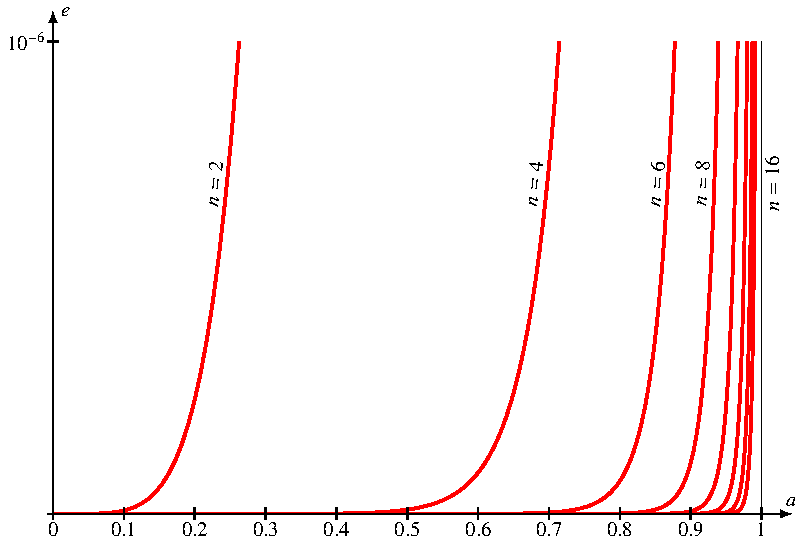
\includegraphics{chapters/060-integral/gq/gq.pdf}
\caption{Approximationsfehler des
Integrals~\eqref{buch:integral:gaussquadratur:bspintegral}
in Abhängigkeit von $a$.
Die Divergenz der Ableitung des Integranden an den Intervallenden
$\pm 1$ führt zu schlechter Konvergenz des Verfahrens, wenn $a$
nahe an $1$ ist.
\label{buch:integral:gaussquadratur:fehler}}
\end{figure}

Zur Illustration der Genauigkeit der Gauss-Quadratur berechnen wir
das Integral
\begin{equation}
\int_{-a}^a \sqrt{1-x^2}\,dx
=
\arcsin a + a \sqrt{1-a^2}
\label{buch:integral:gaussquadratur:bspintegral}
\end{equation}
mit Gauss-Quadratur einerseits und dem Trapezverfahren
andererseits.
Da Gauss-Quadratur mit sehr viel weniger Sützstellen auskommt,
berechnen wir die Trapeznäherung mit zehnmal so vielen Stützstelln.
In den Tabellen~\ref{buch:integral:gaussquadratur:table0.5}
und
\ref{buch:integral:gaussquadratur:table0.999}
sind die Resultate zusammengestellt.
Für $a =\frac12$ zeigt
Tabelle~\ref{buch:integral:gaussquadratur:table0.5}
die sehr schnelle Konvergenz der Gauss-Quadratur, schon mit
12 Stützstellen wird Maschinengenauigkeit erreicht.
Das Trapezverfahren dagegen erreicht auch mit 200 Stützstellen nur
4 korrekte Nachkommastellen.

An den Stellen $x=\pm 1$ divergiert die Ableitung des Integranden
des Integrals \eqref{buch:integral:gaussquadratur:bspintegral}.
Da grösste und kleinste Stützstelle der Gauss-Quadratur immer
deutlich vom Rand des Intervalls entfernt ist, kann das Verfahren
diese ``schwierigen'' Stellen nicht erkennen.
Tabelle~\ref{buch:integral:gaussquadratur:table0.999} zeigt, wie
die Konvergenz des Verfahrens in diesem Fall sehr viel schlechter ist.
Dies zeigt auch der Graph in
Abbildung~\ref{buch:integral:gaussquadratur:fehler}.

\subsection{Skalarprodukte mit Gewichtsfunktion}
Die Nullstellen der Legendre-Polynome ergaben ein gutes
Integrationsverfahren für Polynome auf einem beschränkten
Intervall.
Die Beispiele haben aber auch gezeigt, dass Stellen, wo die
Ableitung des Integranden divergiert, die Genauigkeit stark
beeinträchtigen können.
Ausserdem ist das Verfahren nicht anwendbar auf uneigentliche
Integrale.

\subsubsection{Umgang mit Singularitäten}
Die Lösung des Problems mit Stellen mit divergenter Ableitung
besteht darin, die Stützstellen in der Nähe dieser Stellen
zu konzentrieren.
Die Verwendung einer Gewichtsfunktion $w(x)$ kann genau dies
erreichen.
Statt das Integral einer Funktion $f(x)$ zu bestimmen, 
kann man $f(x)=g(x)w(x)$ schreiben, wobei $w(x)$ so
gewählt werden soll, dass das Verhalten der Steigung an
den Intervallenden gut wiedergibt.
Dies ist mit einer Jacobischen Gewichtsfunktion immer möglich.
Statt der Nullstellen der Legendre-Polynome sind dann die
Nullstellen der Jacobi-Polynome  und die Funktionswete von $g(x)$
an diesen Stellen zu verwenden,  die Gewichte sind
die Integrale von $l_i(x) P^{(\alpha,\beta)}(x)$.

\subsubsection{Uneigentliche Integrale}
Die Berechnung eines uneigentlichen Integrals auf dem Intervall
$(0,\infty)$ oder $(-\infty,\infty)$ ist aus mehreren Gründen nicht
direkt mit dem früher beschriebenen Gauss-Quadraturverfahren
möglich.

Die Stützstellen, die bei der Gauss-Quadratur in einem Intervall
$(a,b)$ verwendet werden, entstehen dadurch, dass man die Nullstellen
der Legendre-Polynome in $(-1,1)$ auf das Intervall $(a,b)$
skaliert.
Dies führt offensichtlich nicht zum Erfolg, wenn ein oder beide
Intervallgrenzen unendlich sind.
Dieses Problem kann dadurch gelöst werden, dass man das unendliche
Intervall $(a,\infty)$ mit
\[
x =  a + \frac{1-t}{t}
\]
auf das Intervall $[0,1]$ transformiert.

Will man beim Intervall $(0,\infty)$ bleiben, dann ist zu beachten,
dass das Integral eines Polynomes immer divergent ist, es ist also
auf jeden Fall nötig, den Integranden durch Funktionen zu approximieren,
die genügend schnell gegen $0$ gehen.
Polynome beliebigen Grades können verwendet werden, wenn sie mit
einer Funktion multipliziert werden, die schneller als jedes Polynom
gegen $0$ geht, so dass das Integral immer noch konvergiert.
Die Funktionen $e^{-x}$ für das Intervall $(0,\infty)$ oder
$e^{-x^2}$ für das Intervall $(-\infty,\infty)$ kommen dafür in Frage.

Um das Integral von $f(x)$ im Intervall $(0,\infty)$ zu berechnen,
schreibt man daher zunächst
\[
\int_0^\infty f(x)\,dx
=
\int_0^\infty g(x)e^{-x}\,dx
=
\int_0^\infty g(x) w(x)\,dx
\quad\text{mit}\quad
w(x)=e^{-x}
\text{ und }
g(x)=f(x)e^x.
\]
Dann approximiert $g(x)$ man durch ein Interpolationspolynom,
so wie man das bei der Gauss-Quadratur gemacht hat.
Als Stützstellen müssen dazu die Nullstellen der Laguerre-Polynome
verwendet werden.
Als Gewichte $w_i$ sind die Integrale der $l_i(x)e^{-x}$
zu verwenden.







%
% rekursion.tex -- drei term rekursion für orthogonale Polynome
%
% (c) 2022 Prof Dr Andreas Müller, OST Ostschweizer Fachhochschule
%
\section{Drei-Term-Rekursion für orthogonale Polynome
\label{buch:orthogonal:section:drei-term-rekursion}}
Die Berechnung der Legendre-Polynome mit Hilfe des Gram-Schmidt-Verfahrens
ist wenig hilfreich, wenn es darum geht, Werte der Polynome zu berechnen.
Glücklicherweise erfüllen orthogonale Polynome automatisch eine 
Rekursionsbeziehung mit nur drei Termen.
Zum Beispiel kann man zeigen, dass für die Legendre-Polynome die
Relation
\begin{align*}
nP_n(x) &= (2n-1)xP_{n-1}(x) - (n-1)P_{n-2}(x),\;\forall n\ge 2,
\\
P_1(x) &= x,
\\
P_0(x) &= 1.
\end{align*}
Mit so einer Rekursionsbeziehung ist es sehr einfach, die Funktionswerte
für alle $P_n(x)$ zu berechnen.

\begin{definition}
Eine Folge von Polynomen $p_n(x)$ heisst orthogonal bezüglich des
Skalarproduktes $\langle\,\;,\;\rangle_w$, wenn 
\[
\langle p_n,p_m\rangle_w = h_n \delta_{nm}
\]
für alle $n$, $m$.
\end{definition}

\subsubsection{Allgemeine Drei-Term-Rekursion für orthogonale Polynome}
Die Multiplikation mit $x$ macht aus einem Polynom vom Grad $n$ ein
Polynom vom Grad $n+1$.
Das Polynom $xp_n(x)$ lässt sich daher als Linearkombination der
Polynome $p_k(x)$ mit $k\le n+1$ schreiben.
Es muss also eine lineare Beziehung zwischen den Polynomen $p_k(x)$ und
$xp_n(x)$ geben, die man nach $p_{n+1}(x)$ auflösen kann, um eine lineare
Darstellung von $p_{n+1}(x)$ durch die $p_k(x)$ und $p_n(x)$ zu
bekommen.
A priori muss man damit rechnen, dass sehr viele Summanden nötig sind.
Der folgende Satz besagt, dass $p_n(x)$ eine Rekursionsbeziehung mit
nur drei Termen erfüllt.

\begin{satz}
\label{buch:orthogonal:satz:drei-term-rekursion}
Eine Folge bezüglich $\langle\,\;,\;\rangle_w$ orthogonaler Polynome $p_n$ 
mit dem Grade $\deg p_n = n$ erfüllt eine Rekursionsbeziehung der Form
\begin{equation}
p_{n+1}(x)
=
(A_nx+B_n)p_n(x) - C_np_{n-1}(x)
\label{buch:orthogonal:eqn:rekursion}
\end{equation}
für $n\ge 0$, wobei $p_{-1}(x)=0$ gesetzt wird.
Die Zahlen $A_n$, $B_n$ und $C_n$ sind reell und es ist
$A_{n-1}A_nC_n\ge 0$ für $n>0$. 
Wenn $k_n>0$ der Leitkoeffizient von $p_n(x)$ ist, dann gilt
\begin{equation}
A_n=\frac{k_{n+1}}{k_n},
\qquad
C_{n+1} = \frac{A_{n+1}}{A_n}\frac{h_{n+1}}{h_n}.
\label{buch:orthogonal:eqn:koeffizientenrelation}
\end{equation}
\end{satz}

Die Rekursionsbeziehung~\eqref{buch:orthogonal:eqn:rekursion} bedeutet,
dass sich die Werte $p_n(x)$ für alle $n$ ausgehend von $p_1(x)$ und
$p_0(x)$ mit nur $O(n)$ Operationen ermitteln lassen.

\subsubsection{Multiplikationsoperator mit $x$}
Man kann die Relation \eqref{buch:orthogonal:eqn:rekursion}
auch nach dem Produkt $xp_n(x)$ auflösen, dann wird sie
\begin{equation}
xp_n(x)
=
\frac{1}{A_n}p_{n+1}(x)
-
\frac{B_n}{A_n}p_n(x)
+
\frac{C_n}{A_n}p_{n-1}(x).
\label{buch:orthogonal:eqn:multixrelation}
\end{equation}
Die Multiplikation mit $x$ ist eine lineare Abbildung im Raum der Funktionen,
die wir weiter unten auch $M_x$ abkürzen.
Die Relation~\eqref{buch:orthogonal:eqn:multixrelation} besagt, dass diese
Abbildung in der Basis der Polynome $p_k$ tridiagonale Form hat.
Ein Beispiel dafür ist im nächsten Abschnitt in
\eqref{buch:orthogonal:eqn:Mx}

\subsubsection{Drei-Term-Rekursion für die Tschebyscheff-Polynome}
Eine Relation der Form~\eqref{buch:orthogonal:eqn:multixrelation}
wurde bereits in 
Abschnitt~\ref{buch:potenzen:tschebyscheff:rekursionsbeziehungen}
hergeleitet.
In der Form~\eqref{buch:orthogonal:eqn:rekursion} geschrieben lautet
sie
\[
T_{n+1}(x) = 2x\,T_n(x)-T_{n-1}(x),
\]
also
$A_n=2$, $B_n=0$ und $C_n=1$.
Die Matrixdarstellung des Multiplikationsoperators $M_x$ in der
Basis der Tschebyscheff-Polynome hat wegen
\eqref{buch:orthogonal:eqn:multixrelation} die Form
\begin{equation}
M_x
=
\begin{pmatrix}
      0&\frac12&      0&      0&      0&\dots  \\
\frac12&      0&\frac12&      0&      0&\dots  \\
      0&\frac12&      0&\frac12&      0&\dots  \\
      0&      0&\frac12&      0&\frac12&\dots  \\
      0&      0&      0&\frac12&      0&\dots  \\
 \vdots& \vdots& \vdots& \vdots& \vdots&\ddots 
\end{pmatrix}.
\label{buch:orthogonal:eqn:Mx}
\end{equation}

\subsubsection{Beweis von Satz~\ref{buch:orthogonal:satz:drei-term-rekursion}}
Die Relation~\eqref{buch:orthogonal:eqn:multixrelation} zeigt auch,
dass der Beweis die Koeffizienten $\langle xp_k,p_j\rangle_w$
berechnen muss.
Dabei wird wiederholt der folgende Trick verwendet.
Für jede beliebige Funktion $f$ mit $\|f\|_w^2<\infty$ ist
\[
\langle fp_k,p_j\rangle_w
=
\langle p_k,fp_j\rangle_w.
\]
Für $f(x)=x$ kann man weiter verwenden, dass $xp_k(x)$ ein Polynom
vom Grad $k+1$ ist.
Die Gleichheit $\langle xp_k,p_j\rangle_w=\langle p_k,xp_j\rangle_w$
ermöglicht also, den Faktor $x$ dorthin zu schieben, wo es nützlicher ist.

\begin{proof}[Beweis des Satzes]
Multipliziert man die rechte Seite von
\eqref{buch:orthogonal:eqn:rekursion} aus, dann ist der einzige Term
vom Grad $n+1$ der Term $A_nxp_n(x)$.
Der Koeffizient $A_n$ ist also dadurch festgelegt, dass
\begin{equation}
b(x)
=
p_{n+1}(x) - A_nxp_n(x)
\label{buch:orthogonal:rekbeweis}
\end{equation}
Grad $\le n$ hat.
Dazu müssen sich die Terme vom Grad $n+1$ in den Polynomen wegheben,
d.~h.~$k_{n+1}-A_nk_n=0$, woraus die erste Beziehung in
\eqref{buch:orthogonal:eqn:koeffizientenrelation} folgt.

Die Polynome $p_k$ sind durch Orthogonalisierung der Monome
$1$, $x$,\dots $x^{k}$ entstanden.
Dies bedeutet, dass $\langle p_n,x^k\rangle_w=0$ für alle $k<n$
gilt und daher auch $\langle p_n,Q\rangle_w=0$ für jedes Polynome
$Q(x)$ vom Grad $<n$.

Das Polynom $b(x)$ ist vom Grad $\le n$, es lässt sich also als
Linearkombination
\[
b(x) = \sum_{k=0}^n b_k p_k(x)
\]
der $p_k$ mit $k\le n$ schreiben.
Die Koeffizienten $b_j$ kann man erhalten, indem man 
\eqref{buch:orthogonal:rekbeweis} Skalar mit $p_j$ multipliziert.
Dabei erhält man
\[
h_jb_j
=
\langle b,p_j\rangle_w
=
\langle p_{n+1},p_j\rangle_w
-
A_n\langle xp_n,p_j\rangle_w.
\]
Für $j\le n$ verschwindet der erste Term nach der Definition einer
Folge von orthogonalen Polynomen.
Den zweiten Term kann man umformen in
\[
\langle xp_n,p_j\rangle_w
=
\langle p_n,xp_j\rangle_w.
\]
Darin ist $xp_j$ ein Polynom vom Grad $j+1$.
Für $n>j+1$ folgt, dass der zweite Term verschwindet.
Somit sind alle $b_j=0$ mit $j<n-1$, nur der Term $j=n-1$
bleibt bestehen.
Mit $B_n=b_n$ und $C_n=b_{n-1}$ bekommt man die somit die
Rekursionsbeziehung~\eqref{buch:orthogonal:eqn:rekursion}.

Indem man das Skalarprodukt von~\eqref{buch:orthogonal:eqn:rekursion}
mit $p_{n-1}$ bildet, findet man
\begin{align}
\underbrace{\langle
p_{n+1},p_{n-1}
\rangle_w}_{\displaystyle=0}
&=
\langle (A_nx+B_n)p_n+C_np_{n-1},p_{n-1} \rangle_w
\notag
\\
0
&=
A_n\langle xp_n,p_{n-1} \rangle_w
+B_n\underbrace{\langle p_n,b_{n-1}\rangle_w}_{\displaystyle=0}
-C_n\|p_{n-1}\|_w^2
\notag
\\
0
&=
A_n\langle p_n,xp_{n-1} \rangle_w
-C_n\|p_{n-1}\|_w^2
\label{buch:orthogonal:eqn:rekbeweis2}
\end{align}
Indem man $xp_n$ als
\[
xp_{n-1}(x)
=
\frac{k_{n-1}}{k_n} p_n(x)
+
\sum_{k=0}^{n-1} d_kp_k(x)
\]
schreibt, bekommt man
\begin{align*}
\langle
p_n,
xp_{n-1}
\rangle_w
&=
\biggl\langle
p_n,
\frac{k_{n-1}}{k_n} p_n
+
\sum_{k=0}^{n-1} d_kp_k
\biggr\rangle_w
=
\frac{k_{n-1}}{k_n}h_n
+
\sum_{k=0}^{n-1} d_k\underbrace{\langle p_n,p_k\rangle_w}_{\displaystyle=0}
\end{align*}
Eingesetzt in~\eqref{buch:orthogonal:eqn:rekbeweis2} erhält man
\[
A_n\frac{k_{n-1}}{k_n}h_n = C_n h_{n-1}
\qquad\Rightarrow\qquad
C_n
=
A_n\frac{k_{n-1}}{k_n}\frac{h_n}{h_{n-1}},
\]
damit ist auch die zweite Beziehung von
\eqref{buch:orthogonal:eqn:koeffizientenrelation}.
\end{proof}

%
% rodrigues.tex
%
% (c) 2022 Prof Dr Andreas Müller, OST Ostschweizer Fachhochschule
%
\section{Rodrigues-Formeln
\label{buch:orthogonalitaet:section:rodrigues}}
Die Drei-Term-Rekursionsformel ermöglicht Werte orthogonaler Polynome
effizient zu berechnen.
Die Rekursionsformel erhöht den Grad eines Polynoms, indem mit $x$ 
multipliziert wird.
mit der Ableitung kann man den Grad aber auch senken, man könnte daher
auch nach einer Rekursionsformel fragen, die bei einem Polynom hohen
Grades beginnt und mit Hilfe von Ableitungen zu geringeren Graden
absteigt.
Solche Formeln heissen Rodrigues-Formeln nach dem Entdecker Olinde
Rodrigues, der eine solche Formal als erster für Legendre-Polynome
gefunden hat.

In diesem Abschnitt sei $p_n(x)$ eine bezüglich des Skalarproduktes
$\langle\,\;,\;\rangle_w$ auf dem Intervall $[a,b]$ orthogonale Familie
von Polynomen mit genaum dem Grad $\deg p_n=n$.
Die Skalarprodukte sollen 
\[
\langle p_n,p_m\rangle_w = h_n\delta_{nm}
\]
sein.

\subsection{Pearsonsche Differentialgleichung}
Die {\em Pearsonsche Differentialgleichung} ist die Differentialgleichung
\begin{equation}
B(x) y' - A(x) y = 0,
\label{buch:orthogonal:eqn:pearson}
\end{equation}
wobei $B(x)$ ein Polynom vom Grad höchstens $2$ ist und $A(x)$ ein
höchstens lineares Polynom.
Die Gleichung~\eqref{buch:orthogonal:eqn:pearson}
kann gelöst werden, wenn $y$ und $B(x)$ keine Nullstellen  haben.
Dann kann man die Gleichung umstellen in
\[
\frac{y'}{y}
=
(\log y)'
=
\frac{A(x)}{B(x)}
\qquad\Rightarrow\qquad
y = \exp\biggl( \int\frac{A(x)}{B(x)}\biggr)\,dx.
\]
Im folgenden nehmen wir zusätzlich an, dass
\begin{equation}
\lim_{x\to a+} w(x)B(x) = 0,
\qquad\text{und}\qquad
\lim_{x\to b-} w(x)B(x) = 0.
\end{equation}
Falls $w(x)$ an den Intervallenden einen von $0$ verschiedenen
Grenzwert hat, bedeutet dies, dass $B(a)=B(b)=0$ sein muss.
Falls $w(x)$ am Intervallende divergiert, muss $B(x)$ dort eine
Nullstelle höherer Ordnung haben, was aber für ein Polynom
zweiten Grades nicht möglich ist.

\subsection{Rekursionsformel}
Multiplikation mit $B(x)$ wird den Grad eines Polynomes typischerweise 
um $2$ erhöhen, die Ableitung wird ihn wieder um $1$ reduzieren.
Etwas formeller kann man dies wie folgt formulieren:

\begin{satz}
Für alle $n\ge 0$ ist
\[
q_n(x)
=
\frac{1}{w(x)}
\frac{d^n}{dx^n} B(x)^n w(x)
\]
ein Polynom vom Grad höchstens $n$.
\end{satz}

\begin{proof}[Beweis]
Wenn $r_0(x)$ irgend eine differenzierbare Funktion ist, dann ist
\begin{align*}
\frac{d^n}{dx^n}
r_0(x) B(x)^n w(x)
&=
\frac{d^{n-1}}{dx^{n-1}}\frac{d}{dx} r_0(x) B(x)^n w(x)
\\
&=
\frac{d^{n-1}}{dx^{n-1}}
\bigl(r_0'(x)B(x)+ nB'(x)B(x)^{n-1}w(x) + B(x)^n w'(x) \bigr)
\\
&=
\frac{d^{n-1}}{dx^{n-1}}
(r_0'(x)B(x)+nB'(x)+A(x)) B(x)^{n-1} w(x)
=
\frac{d^{n-1}}{dx^{n-1}} r_1(x)B^{n-1}(x) w(x).
\end{align*}
Für die Funktionen $r_k$ gilt die Rekursionsformel
\begin{equation}
r_k(x) = r_{k-1}'(x)B(x) + kB'(x) + A(x).
\label{buch:orthogonal:rodrigues:rekursion:beweis1}
\end{equation}
Wenn $r_0(x)$ ein Polynom ist, dann sind alle Funktionen $r_k(x)$
ebenfalls Polynome.
Durch wiederholte Anwendung dieser Formel kann man schliessen, dass 
\[
\frac{d^n}{dx^n} r_0(x) B(x)^n w(x)
=
r_n(x) w(x).
\]
Insbesondere folgt für $r_0(x)=1$, dass man durch $w(x)$ dividieren kann
und dass $r_n(x)=q_n(x)$.

Wir müssen auch noch den Grad von $r_k(x)$ bestimmen.
Dazu verwenden wir 
\eqref{buch:orthogonal:rodrigues:rekursion:beweis1} und berechnen den
Grad:
\begin{equation*}
\deg r_k(x)
=
\max \bigl(
\underbrace{\deg(r_{k-1}'(x) B(x))}_{\displaystyle \deg r_{k-1}(x) -1 + 2}
,
\underbrace{\deg(B'(x))}_{\displaystyle \le 1}
,
\underbrace{\deg(A(x))}_{\displaystyle \le 1}
\bigr)
\le \max r_{k-1}(x) + 1.
\end{equation*}
Aus $\deg r_0(x)=0$ kann man jetzt ablesen, dass $\deg r_k(x)\le k$ ist.
Damit ist gezeigt, dass $\deg q_n(x)\le n$.
\end{proof}

\begin{satz}
Es gibt Konstanten $c_n$ derart, dass
\[
p_n(x)
=
\frac{c_n}{w(x)} \frac{d^n}{dx^n} \bigl(B(x)^n w(x)\bigr) 
\]
gilt.
\end{satz}

\begin{proof}[Beweis]
Wir müssen zeigen, dass die Polynome orthogonal sind auf allen Monomen
von geringerem Grad.
\begin{align*}
\langle q_n, x^k\rangle_w
&=
\int_a^b q_n(x)x^kw(x)\,dx
\\
&=
\int_a^b \frac{1}{w(x)}\frac{d^n}{dx^n}(B(x)^n w(x)) x^k w(x)\,dx
\\
&=
\int_a^b \frac{d^n}{dx^n}(B(x)^n w(x)) x^k \,dx
\\
&=
\biggl[\frac{d^{n-1}}{dx^{n-1}}(B(x)^n w(x)) x^k \biggr]_a^b
-
\int_a^b \frac{d^{n-1}}{dx^{n-1}}(B(x)^n w(x))kx^{k-1}\,dx
\end{align*}
Durch $n$-fache Iteration wird das Integral auf $0$ reduziert.
Es bleiben nur die eckigen Klammern stehen, doch wenn man die Produktregel
auswertet, bleibt immer mindestens ein Produkt $B(x)w(x)$ stehen,
nach den Voraussetzungen an den Grenzwert dieses Produktes an den
Intervallenden verschwinden diese Terme alle.
Damit sind die $q_n(x)$ Polynome, die $w$-orthogonal sind auf allen
$x^k$ mit $k<n$, also Vielfache der $w$-Orthgonalpolynome.
\end{proof}

\subsubsection{Legendre-Polynome}
Legendre-Polynome sind orthogonale Polynome zum Standardskalarprodukt
mit $w(x)=1$.
Die Pearsonsche Differentialgleichung ist für $A(x)=0$ immer erfüllt.
Die Randbedingung bedeutet wegen $w(x)=1$, dass $B(x)$ an den
Endpunkten des Intervalls verschwinden muss.
Da $B(x)$ ein Polynom höchstens vom Grad $2$ ist, muss $B(x)$ ein
Vielfaches von $(x-1)(x+1)=x^-1$ sein.
Die Rodrigues-Formel für die Legendre-Polynome hat daher die Form
\[
P_n(x)
=
c_n
\frac{d^n}{dx^n}
(x^2-1)^n,
\]
darin müssen die Konstanten $c_n$ noch bestimmt werden.
In der für die Legendre-Polynome gewählten Normierung ist
\[
c_n = \frac1{2^n n!}
\qquad\text{und damit}\qquad
P_n(x)
=
\frac{1}{2^nn!}
\frac{d^n}{dx^n}
(x^2-1)^n.
\]

\subsubsection{Hermite-Polynome}
TODO

\url{https://en.wikipedia.org/wiki/Rodrigues%27_formula}



%
% legendredgl.tex
%
% (c) 2021 Prof Dr Andreas Müller, OST Ostschweizer Fachhochschule
%
\subsection{Orthogonale Polynome und Differentialgleichungen}
Legendre hat einen ganz anderen Zugang zu den nach ihm benannten
Polynomen gefunden.
Er hat sie gefunden als die Lösungen einer speziellen Differentialgleichungen.
In diesem Abschnitt sollen diese Funktionen mit der Potenzreihen-Methode
wiedergefunden werden.
Dabei stellt sich heraus, dass diese Polynome auch Eigenfunktionen eines
selbstadjungierten Differentialgoperator sind.
Die Orthogonalität wird dann aus einer Verallgemeinerung der bekannten
Eingeschaft folgen, dass Eigenvektoren einer symmetrischen Matrix zu 
verschiedenen Eigenwerten orthogonal sind.

\subsubsection{Legendre-Differentialgleichung}
Die {\em Legendre-Differentialgleichung} ist die Differentialgleichung
\begin{equation}
(1-x^2) y'' - 2x y' + n(n+1) y = 0
\label{buch:integral:eqn:legendre-differentialgleichung}
\end{equation}
für eine Funktion $y(x)$ auf dem Intervall $[-1,1]$.

Sei $y(x)$ eine Lösung der Differentialgleichung
\eqref{buch:integral:eqn:legendre-differentialgleichung}.
Setzt man $y_s(x)=y(-x)$ in die Differentialgleichung ein, erhält
man
\[
(1-x^2)y_s''(x) - 2x y'_s(x) + n(n+1)y_s(x)
=
(1-x^2)y''(-x) +2x y(-x) +n(n+1)y(-x).
\]
Ersetzt man $t=-x$, dann wird daraus
\[
(1-x^2)y''(t) -2t y(t) + n(n+1) y(t) = 0
\]
aus der Differentialgleichung
\eqref{buch:integral:eqn:legendre-differentialgleichung}.
Insbesondere ist die gespiegelte Funktion $y_s(x)$ ebenfalls
eine Lösung der Differentialgleichung.

Ist $y(x)$ eine Lösung der Differentialgleichung ist, dann lässt
sie sich in die Summe einer geraden und einer ungeraden Funktion
\[
\left.
\begin{aligned}
y_g(x) &= \frac{y(x)+y(-x)}{2}\\
y_u(x) &= \frac{y(x)-y(-x)}{2}
\end{aligned}
\quad
\right\}
\quad
\Rightarrow
\quad
y(x) = y_g(x) + y_u(x)
\]
zerlegen, die als Linearkombinationen der beiden Lösungen
$y(x)$ und $y_s(x)$ ebenfalls Lösungen der Differentialgleichung
sind.

\subsubsection{Potenzreihenlösung}
Wir suchen eine Lösung in Form einer Potenzreihe um $x=0$ und 
verwenden dazu den Ansatz
\[
y(x) = a_0+a_1x+a_2x^2+ \dots = \sum_{k=0}^\infty a_kx^k.
\]
\begin{align*}
(1-x^2) \sum_{k=2}^\infty k(k-1)a_kx^{k-2}
-2x\sum_{k=0}^\infty ka_kx^{k-1}
+
n(n+1)\sum_{k=0}^\infty  a_kx^k
&=
0
\\
\sum_{k=0}^\infty (k+2)(k+1)a_{k+2}x^k
-
\sum_{k=2}^\infty k(k-1)a_kx^k
-
2\sum_{k=1}^\infty ka_kx^k
+
n(n+1)\sum_{k=0}^\infty  a_kx^k
&=
0
\end{align*}
Die Koeffizienten zur Potenz $k$ sind daher
\begin{align}
k&=0:
&
0&=
2a_2+n(n+1)a_0
\notag
\\
&&
a_2&=-\frac{n(n+1)}{2}a_0
\notag
\\
k&=1:
&
0&=
6a_3-2a_1+n(n+1)a_1
\notag
\\
&&
a_3&= \frac{2-n(n+1)}{6}a_1
\notag
\\
k&>1:
&
0&=
(k+2)(k+1)a_{k+2} -k(k-1)a_k -2ka_k +n(n+1) a_k
\notag
\\
&&
a_{k+2}
&=
\frac{ k(k+1)-n(n+1) }{(k+2)(k+1)}
a_k
\label{buch:integral:legendre-dgl:eqn:akrek}
\end{align}
Wenn $a_1=0$ und $a_0\ne 1$ ist, dann ist die Funktion $y(x)$ gerade,
alle ungeraden Koeffizienten verschwinden.
Ebenso verschwinden alle geraden Koeffizienten, wenn $a_0=0$ und $a_1\ne 0$.
Für jede Lösung $y(x)$ der Differentialgleichung ist
$y_g(x)$ ein Lösung mit $a_1=0$ und $y_u(x)$ eine Lösung mit $a_0=0$.
Wir können die Diskussion der Lösungen daher auf gerade oder ungerade
Lösungen einschränken.

Gesucht ist jetzt eine Lösung in Form eines Polynoms.
In diesem Fall müssen die Koeffizienten $a_k$ ab einem
gewissen Index verschwinden.
Dies tritt nach \eqref{buch:integral:legendre-dgl:eqn:akrek} genau
dann auf, wenn der Zähler für ein $k$ verschwindet.
Folglich gibt es genau dann Polynomlösungen der Differentialgleichungen,
wenn $n$ eine natürlich Zahl ist.
Ausserdem ist die Lösung ein Polynom $\bar{P}_n(x)$ vom Grad $n$.
Das Polynom soll wieder so normiert sein, dass $\bar{P}_n(1)=1$ ist.

Die Lösungen der Differentialgleichungen können jetzt explizit
berechnet werden.
Zunächst ist $\bar{P}_0(x)=1$ und $\bar{P}_1(x)=x$.
Für $n=2$ setzen wir zunächst $a_0=1$ und $a_1=0$ und erhalten
\[
y(x)
=
1 + \frac{0(0+1) - 2(2+1)}{(0+2)(0+1)}a_0 x^2
=
1
-3x^2
\qquad\text{oder}\qquad
\bar{P}_3(x) = \frac12(3x^2-1).
\]
Für $n=3$ starten wir von $a_1=1$ und $a_0=0$, was zunächst $a_2=0$
impliziert.
Für $a_3$ finden wir
\[
a_3=\frac{1(1+1)-3(3+1)}{(1+2)(1+1)} = -\frac53
\qquad\Rightarrow\qquad
y(x) = x-\frac53x^3
\qquad\Rightarrow\qquad
\bar{P}_3(x) = \frac12(5x^3-3x).
\]
Dies stimmt überein mit den früher gefundenen Ausdrücken für
die Legendre-Polynome.

Die Potenzreihenlösung zeigt zwar, dass es für jedes $n\in\mathbb{N}$
eine Polynomlösung $\bar{P}_n(x)$ vom Grad $n$ gibt.
Dies kann aber nicht erklären, warum die so gefundenen Polynome
orthogonal sind.

\subsubsection{Eigenfunktionen}
Die Differentialgleichung
\eqref{buch:integral:eqn:legendre-differentialgleichung}
Kann mit dem Differentialoperator
\[
D = \frac{d}{dx}(1-x^2)\frac{d}{dx}
\]
als
\[
Dy + n(n+1)y = 0
\]
geschrieben werden.
Tatsächlich ist
\[
Dy
=
\frac{d}{dx} (1-x^2) \frac{d}{dy}
=
\frac{d}{dx} (1-x^2)y'
=
(1-x^2)y'' -2x y'.
\]
Dies bedeutet, dass die Lösungen $\bar{P}_n(x)$ Eigenfunktionen
des Operators $D$ zum Eigenwert $n(n+1)$ sind:
\[
D\bar{P}_n = -n(n+1) \bar{P}_n.
\]

\subsubsection{Orthogonalität von $\bar{P}_n$ als Eigenfunktionen}
Ein Operator $A$ auf Funktionen heisst {\em selbstadjungiert}, wenn
für zwei beliebige Funktionen $f$ und $g$ gilt
\[
\langle Af,g\rangle = \langle f,Ag\rangle
\]
gilt.
Im vorliegenden Zusammenhang möchten wir die Eigenschaft nutzen,
dass Eigenfunktionen eines selbstadjungierten Operatores zu verschiedenen
Eigenwerten orthogonal sind.
Dazu seien $Df = \lambda f$ und $Dg=\mu g$ und wir rechnen
\begin{equation*}
\renewcommand{\arraycolsep}{2pt}
\begin{array}{rcccrl}
\langle Df,g\rangle &=& \langle \lambda f,g\rangle &=& \lambda\phantom{)}\langle f,g\rangle
&\multirow{2}{*}{\hspace{3pt}$\biggl\}\mathstrut-\mathstrut$}\\
=\langle f,Dg\rangle &=& \langle f,\mu g\rangle &=& \mu\phantom{)}\langle f,g\rangle&
\\[2pt]
\hline
         0           & &                        &=& (\lambda-\mu)\langle f,g\rangle&
\end{array}
\end{equation*}
Da $\lambda-\mu\ne 0$ ist, muss $\langle f,g\rangle=0$ sein.

Der Operator $D$ ist selbstadjungiert, d.~h.
für zwei beliebige zweimal stetig differenzierbare Funktion $f$ und $g$
auf dem Intervall $[-1,1]$ gilt
\begin{align*}
\langle Df,g\rangle
&=
\int_{-1}^1 (Df)(x) g(x) \,dx
\\
&=
\int_{-1}^1
\biggl(\frac{d}{dx} (1-x^2)\frac{d}{dx}f(x)\biggr) g(x)
\,dx
\\
&=
\underbrace{
\biggl[
\biggl((1-x^2)\frac{d}{dx}f(x)\biggr) g(x)
\biggr]_{-1}^1
}_{\displaystyle = 0}
-
\int_{-1}^1
\biggl((1-x^2)\frac{d}{dx}f(x)\biggr) \frac{d}{dx}g(x)
\,dx
\\
&=
-
\int_{-1}^1
\biggl(\frac{d}{dx}f(x)\biggr) \biggl((1-x^2)\frac{d}{dx}g(x)\biggr)
\,dx
\\
&=
-
\underbrace{
\biggl[
f(x) \biggl((1-x^2)\frac{d}{dx}g(x)\biggr)
\biggr]_{-1}^1}_{\displaystyle = 0}
+
\int_{-1}^1
f(x) \biggl(\frac{d}{dx}(1-x^2)\frac{d}{dx}g(x)\biggr)
\,dx
\\
&=
\langle f,Dg\rangle.
\end{align*}
Dies beweist, dass $D$ selbstadjungiert ist.
Da $\bar{P}_n$ Eigenwerte des selbstadjungierten Operators $D$ zu
den verschiedenen Eigenwerten $-n(n+1)$ sind, folgt auch, dass
die $\bar{P}_n$ orthogonale Polynome vom Grad $n$ sind, die die 
gleiche Standardierdisierungsbedingung wie die Legendre-Polyonome
erfüllen, also ist $\bar{P}_n(x)=P_n(x)$.

\subsubsection{Legendre-Funktionen zweiter Art}
%Siehe Wikipedia-Artikel \url{https://de.wikipedia.org/wiki/Legendre-Polynom}
%
Die Potenzreihenmethode liefert natürlich auch Lösungen der
Legendreschen Differentialgleichung, die sich nicht als Polynome
darstellen lassen.
Ist $n$ gerade, dann liefern die Anfangswerte $a_0=0$ und $a_1=1$ 
eine ungerade Funktion, die Folge der Koeffizienten bricht
aber nicht ab, vielmehr ist
\begin{align*}
a_{k+2}
&=
\frac{k(k+1)}{(k+1)(k+2)}a_k
=
\frac{k}{k+2}a_k.
\end{align*}
Durch wiederholte Anwendung dieser Rekursionsformel findet man
\[
a_{k}
=
\frac{k-2}{k}a_{k-2}
=
\frac{k-2}{k}\frac{k-4}{k-2}a_{k-4}
=
\frac{k-2}{k}\frac{k-4}{k-2}\frac{k-6}{k-4}a_{k-6}
=
\dots
=
\frac{1}{k}a_1.
\]
Die Lösung hat daher die Reihenentwicklung
\[
Q_0(x) = x+\frac13x^3 + \frac15x^5 + \frac17x^7+\dots
=
\frac12\log \frac{1+x}{1-x}
=
\operatorname{artanh}x.
\]
Die Funktion $Q_0(x)$ heisst {\em Legendre-Funktion zweiter Art}.

Für $n=1$ wird die Reihenentwicklung $a_0=1$ und $a_1=0$ etwas
interessanter.
Die Rekursionsformel für die Koeffizienten ist
\[
a_{k+2}
=
\frac{k(k+1)-2}{(k+1)(k+2)} a_k.
\qquad\text{oder}\qquad
a_k
=
\frac{(k-1)(k-2)-2}{k(k-1)}
a_{k-2}
\]
Man erhält der Reihe nach
\begin{align*}
a_2 &= \frac{-2}{2\cdot 1} a_0 = -1
\\
a_3 &= 0
\\
a_4 &= \frac{3\cdot 2-2}{4\cdot 3} a_2 = \frac{4}{4\cdot 3}a_2 = \frac13a_2 = -\frac13
\\
a_5 &= 0
\\
a_6 &= \frac{5\cdot 4-2}{6\cdot 5}a_4 = \frac{18}{6\cdot 5}a_4 = -\frac15
\\
a_7 &= 0
\\
a_8 &= \frac{7\cdot 6-2}{8\cdot 7}a_6 = \frac{40}{8\cdot 7} = -\frac17
\\
a_9 &= 0
\\
a_{10} &= \frac{9\cdot 8-2}{10\cdot 9}a_8 = \frac{70}{10\cdot 9} = -\frac19,
\end{align*}
woraus sich die Reihenentwicklung
\begin{align*}
y(x)
&=
-x^2 -\frac13x^4 -\frac15x^6 - \frac17x^8 -\frac19x^{10}-\dots
\\
&=
-x\biggl(x+\frac13x^3 + \frac15x^5 + \frac17x^7 + \frac19x^9+\dots\biggr)
=
-x\operatorname{artanh}x.
\end{align*}
Die {\em Legendre-Funktionen zweiter Art} $Q_n(x)$  werden allerdings
so definiert, dass gewisse Rekursionsformeln für die Legendre-Polynome,
die wir hier nicht hergeleitet haben, auch für die $Q_n(x)$ gelten.
In dieser Normierung muss statt des eben berechneten $y(x)$ die Funktion
\[
Q_1(x) = x \operatorname{artanh}x-1
\]
verwendet werden.







%
% bessel.tex
%
% (c) 2021 Prof Dr Andreas Müller, OST Ostschweizer Fachhochschule
%
\section{Bessel-Funktionen
\label{buch:differntialgleichungen:section:bessel}}
\rhead{Bessel-Funktionen}
Die Besselsche Differentialgleichung
erlaubt Wellen mit zylindrischer
Symmetrie und die Strömung in einem zylindrischen Rohr zu beschreiben.
Die Auflösung eines optischen Systems wird durch die Beugung limitiert,
die Helligkeitskverteilung des Bildes einer Punktquelle ist
zylindersymmetrisch und kann mit Hilfe von Lösungen der Besselschen
Differentialgleichung beschrieben werden.
Die Besselsche Differentialgleichung hat im Allgemeinen keine Lösung,
die sich durch bekannte Funktionen ausdrücken lassen, es ist also
nötig, eine neue Familie von speziellen Funktionen zu definieren,
die Bessel-Funktionen.

%
% Besselsche Differentialgleichung
%
\subsection{Die Besselsche Differentialgleichung}
% XXX Wo taucht diese Gleichung auf
Die Besselsche Differentialgleichung ist die Differentialgleichung
\begin{equation}
x^2\frac{d^2y}{dx^2} + x\frac{dy}{dx} + (x^2-\alpha^2)y = 0
\label{buch:differentialgleichungen:eqn:bessel}
\end{equation}
zweiter Ordnung
für eine auf dem Interval $[0,\infty)$ definierte Funktion $y(x)$.
Der Parameter $\alpha$ ist eine beliebige komplexe Zahl $\alpha\in \mathbb{C}$,
die Lösungsfunktionen hängen daher von $\alpha$ ab.

%
% Eigenwertproblem
%
\subsubsection{Eigenwertproblem}
Die Besselsche Differentialgleichung
\eqref{buch:differentialgleichungen:eqn:bessel}
kann man auch als Eigenwertproblem für den Bessel-Operator
\index{Bessel-Operator}%
\begin{equation}
B = x^2\frac{d^2}{dx^2} + x\frac{d}{dx} + x^2
\label{buch:differentialgleichungen:bessel-operator}
\end{equation}
schreiben.
Eine Lösung $y(x)$ der Gleichung
\eqref{buch:differentialgleichungen:eqn:bessel}
erfüllt
\[
By
=
x^2y''+xy'+x^2y
=\alpha^2 y,
\]
ist also eine Eigenfunktion des Bessel-Operators zum Eigenwert
$\alpha^2$.

%
% Indexgleichung
%
\subsubsection{Indexgleichung}
Die Besselsche Differentialgleichung ist eine Differentialgleichung
der Art~\eqref{buch:differentialgleichungen:eqn:dglverallg} mit
\[
p(x) = 1
\qquad\text{und}\qquad
q(x) = x^2-\alpha^2.
\]
Nach den Ausführungen von
Abschnitt~\ref{buch:differentialgleichungen:subsection:verallgemeinrt},
muss die Lösung in der Form einer verallgemeinerten Potenzreihe 
gesucht werden.
Dazu muss zunächst die Indexgleichung
\[
0
=
X(X-1) + Xp_0 + q_0
=
X(X-1) + X - \alpha^2
=
X^2-\alpha^2
=
(X-\alpha)(X+\alpha)
\]
gelöst werden.
Die Nullstellen sind offenbar $\varrho_1=\alpha$ und $\varrho_2=-\alpha$.

Die beiden Vorzeichen der Nullstellen der Indexgleichung führen
auf die gleiche Differentialgleichung.
Der Lösungsraum der Differentialgleichung ist natürlich trotzdem
zweidimensional, so dass es immer noch möglich ist, den
beiden Nullstellen der Indexgleichung verschiedene Lösungen
zuzuordnen.
Die Diskussion in
Abschnitt~\ref{buch:differentialgleichungen:subsection:verallgemeinrt}
hat Kriterien ergeben, unter denen zwei linear unabhängige Lösungen
mit Hilfe einer verallgemeinerten Potenzreihe gefunden werden können.
Falls nur eine solche Lösung gefunden werden kann, wird sie der grösseren
der beiden Zahlen $\alpha$ und $-\alpha$ zugeordnet
(oder $0$, falls $\alpha=-\alpha=0$).
Eine weitere Lösung kann mit Hilfe analytischer Fortsetzung gefunden werden,
wie später gezeigt wird.

Für nicht reelles $\alpha$ kann $\varrho_1-\varrho_2=2\alpha$ keine 
Ganzzahl sein, es ist also garantiert, dass zwei linear unabhängig
Lösungen der Form
\begin{equation}
y_1(x) = x^\alpha\sum_{k=0}^\infty a_kx^k
\qquad\text{und}\qquad
y_2(x) = x^{-\alpha}\sum_{k=0}^\infty b_kx^k.
\label{buch:differentialgleichungen:eqn:besselloesungen}
\end{equation}
existieren.

Für reelles $\alpha\in\mathbb{R}$ gibt es zwei Lösungen der
Form~\eqref{buch:differentialgleichungen:eqn:besselloesungen}
genau dann, wenn $\varrho_1-\varrho_2$ keine Ganzzahl ist.
Nur eine Lösung kann man finden, wenn 
\[
\alpha-(-\alpha)=2\alpha \in \mathbb{Z}
\qquad\Rightarrow\qquad
\alpha = \frac{k}{2},\quad k\in\mathbb{Z}
\]
ist.

%
% Bessel-Funktionen erster Art
%
\subsection{Bessel-Funktionen erster Art
\label{buch:differentialgleichungen:subsection:bessel1steart}}
Für $\alpha \ge 0$ gibt es immer mindestens eine Lösung der Besselgleichung
als verallgemeinerte Potenzreihe mit $\varrho=\alpha$.
Die Funktion $q(x)=x^2-\alpha^2$ ist ein Polynom, die einzigen
von $0$ verschiedenen Koeffizienten sind $q_0=-\alpha^2$
und $q_2=1$.
Für den ersten Koeffizienten $a_0$ gibt es keine Einschränkungen,
wir wählen $a_0=1$.

Die Rekursionsformel für $n=1$ ist
\[
F(\varrho+1) a_1 = (\varrho p_1+q_1)a_0,
\]
aber die Koeffizienten $p_1$ und $q_1$ verschwinden beide und damit
die ganze rechte Seite.
Da $F(\varrho+1)\ne 0$ ist, folgt dass $a_1=0$ sein muss.

% Fall n=1 gesondert behandeln

%
% Der allgemeine Fall
%
\subsubsection{Der allgemeine Fall}
Für die höheren Potenzen $n>1$ wird die Rekursionsformel für die
Koeffizienten $a_n$ der verallgemeinerten Potenzreihe
\[
a_{n} =
-\frac{ q_2 a_{n-2} }{F(\varrho+n)}
=
-\frac{a_{n-2}}{(\varrho+n)^2-\alpha^2}
=
-\frac{a_{n-2}}{\varrho^2 + 2\varrho n+n^2-\alpha^2}
=
-\frac{a_{n-2}}{n(n+2\varrho)}.
\]
Im letzten Schritt haben wir verwendet, dass $\varrho=\pm\alpha$
und damit $\varrho^2=\alpha^2$ ist.
Daraus folgt wegen $a_1=0$, dass auch $a_{2k+1}=0$ für alle $k$.
Damit können wir jetzt die Reihe hinschreiben:
\begin{align*}
y(x)
&=
x^{\varrho}\biggl(
1
-
\frac{1}{2(2+2\varrho)} x^2
+
\frac{1}{2(2+2\varrho)4(4+2\varrho)} x^4
-
\frac{1}{2(2+2\varrho)4(4+2\varrho)6(6+2\varrho)} x^6
+
\dots
\biggr)
\\
&=
x^{\varrho}
\biggl(
1
+
\frac{(-x^2/4)}{1\cdot (1+\varrho)}
+
\frac{(-x^2/4)^2}{1\cdot 2\cdot (1+\varrho)\cdot(2-\varrho)}
+
\frac{(-x^2/4)^3}{1\cdot 2\cdot 3\cdot (1+\varrho)\cdot(2+\varrho)\cdot(3+\varrho)}
+
\dots
\biggr)
\\
&=
x^\varrho\biggl(
1
+
\frac{1}{(\varrho+1)}\frac{(-x^2/4)}{1!}
+
\frac{1}{(\varrho+1)(\varrho+2)}\frac{(-x^2/4)^2}{2!}
+
\frac{1}{(\varrho+1)(\varrho+2)(\varrho+3)}\frac{(-x^2/4)^3}{3!}
+
\dots
\biggr)
\\
&=
x^\varrho \sum_{k=0}^\infty
\frac{1}{(\varrho+1)_k} \frac{(-x^2/4)}{k!}
=
x^\varrho
\cdot
\mathstrut_0F_1\biggl(;\varrho+1;-\frac{x^2}{4}\biggr)
\end{align*}
Wir finden also zwei Lösungsfunktionen
\begin{align}
y_1(x)
%J_\alpha(x)
&=
x^{\alpha\phantom{-}}
\sum_{k=0}^\infty
\frac{1}{(\alpha+1)_k}
\frac{(-x^2/4)^k}{k!}
=
x^\alpha
\cdot
\mathstrut_0F_1\biggl(;\alpha+1;-\frac{x^2}{4}\biggr),
\label{buch:differentialgleichunge:bessel:eqn:erste}
\\
y_2(x)
%J_{-\alpha}(x)
&=
x^{-\alpha} \sum_{k=0}^\infty
\frac{1}{(-\alpha+1)_k} \frac{(-x^2/4)^k}{k!}
=
x^{-\alpha}
\cdot
\mathstrut_0F_1\biggl(;-\alpha+1;-\frac{x^2}{4}\biggr).
\label{buch:differentialgleichunge:bessel:eqn:zweite}
\end{align}
Man beachte, dass die zweite Lösung für ganzzahliges $\alpha>0$ nicht
definiert ist.
Man kann auch direkt nachrechnen, dass diese Funktionen Lösungen
der Besselschen Differentialgleichung sind.

%
% Bessel-Funktionen
%
\subsubsection{Bessel-Funktionen}
Da die Besselsche Differentialgleichung linear ist, ist auch
jede Linearkombination der Funktionen
\eqref{buch:differentialgleichunge:bessel:eqn:erste}
und
\eqref{buch:differentialgleichunge:bessel:eqn:zweite}
eine Lösung.
Satz~\ref{buch:rekursion:gamma:satz:gamma-pochhammer}
ermöglicht, das Pochhammer-Symbol durch Werte der Gamma-Funktion
wie in
\[
(\alpha+1)_n = \frac{\Gamma(\alpha+k+1)}{\Gamma(\alpha+1)}
\]
auszudrücken.
Damit wird
\begin{align}
y_1(x)
&=
x^\alpha
\sum_{k=0}^\infty
\frac{\Gamma(\alpha+1)}{\Gamma(\alpha+k+1)}
\frac{(-x^2/4)^k}{k!}
=
\Gamma(\alpha+1) 2^{\alpha}
\biggl(\frac{x}{2}\biggr)^\alpha
\sum_{k=0}^\infty
\frac{(-1)^k}{k!\,\Gamma(\alpha+k+1)} \biggl(\frac{x}{2}\biggr)^{2k}
\label{buch:differentialgleichungen:bessel:normierungsgleichung}
\end{align}
Nur gerade der Faktor $2^\alpha\Gamma(\alpha+1)$ ist von $k$ und $x$ 
unabhängig, daher ist die folgende Definition sinnvoll:

\begin{definition}
\label{buch:differentialgleichungen:bessel:definition}
Die Funktion
\[
J_{\alpha}(x)
=
\biggl(\frac{x}{2}\biggr)^\alpha
\sum_{k=0}^\infty
\frac{(-1)^k}{k!\,\Gamma(\alpha+k+1)}
\biggl(\frac{x}{2}\biggr)^{2k}
\]
heisst {\em Bessel-Funktion erster Art der Ordnung $\alpha$}.
\index{Bessel-Funktion!erster Art}%
\end{definition}

Die Bessel-Funktion $J_\alpha(x)$ der Ordnung $\alpha$ unterscheidet sich
nur durch einen Normierungsfaktor von der Lösung $y_1(x)$.
Dasselbe gilt für $J_{-\alpha}(x)$ und $y_2(x)$:
\begin{align*}
J_{\alpha}(x)
&=
\frac{1}{2^\alpha\Gamma(\alpha+1)}
\cdot
y_1(x)
\\
J_{-\alpha}(x)
&=
\frac{1}{2^{-\alpha}\Gamma(-\alpha+1)}
\cdot
y_2(x).
\end{align*}

%
% Ganzzahlige Ordnung
%
\subsubsection{Besselfunktionen ganzzahliger Ordnung}
Man beachte, dass diese Definition für beliebige ganzzahlige 
$\alpha$ funktioniert.
Ist $\alpha=-n<0$, $n\in\mathbb{N}$, dann hat der Nenner Pole 
an den Stellen $k=0,1,\dots,n-1$.
Die Summe beginnt also erst bei $k=n$ oder
\begin{align*}
J_{-n}(x)
&=
\sum_{k=n}^\infty \frac{(-1)^k}{m!\,k!}\biggl(\frac{x}{2}\biggr)^{2k-n}
=
\sum_{l=0}^\infty
\frac{(-1)^{l+n}}{m!\,(l+n)!}\biggl(\frac{x}{2}\biggr)^{2(l+n)-n}
=
(-1)^n
\sum_{l=0}^\infty
\frac{(-1)^l}{m!\,\Gamma(l+n+1)}\biggl(\frac{x}{2}\biggr)^{2l+n}
\\
&=
(-1)^n
J_{n}(x).
\end{align*}
Insbesondere unterscheiden sich $J_n(x)$ und $J_{-n}(x)$ nur durch
ein Vorzeichen.

Als lineare Differentialgleichung zweiter Ordnung erwarten wir noch
eine zweite, linear unabhängige Lösung.
Diese kann jedoch nicht allein mit der Potenzreihenmethode,
dazu sind die Methoden der Funktionentheorie nötig.
Im Abschnitt~\ref{buch:funktionentheorie:subsection:dglsing}
wird gezeigt, wie dies möglich ist und auf
Seite~\pageref{buch:funktionentheorie:subsubsection:bessel2art}
werden die damit zu findenden Bessel-Funktionen 0-ter Ordnung und
zweiter Art vorgestellt.

%
% Erzeugende Funktione
%
\subsubsection{Erzeugende Funktion}
\begin{figure}
\centering
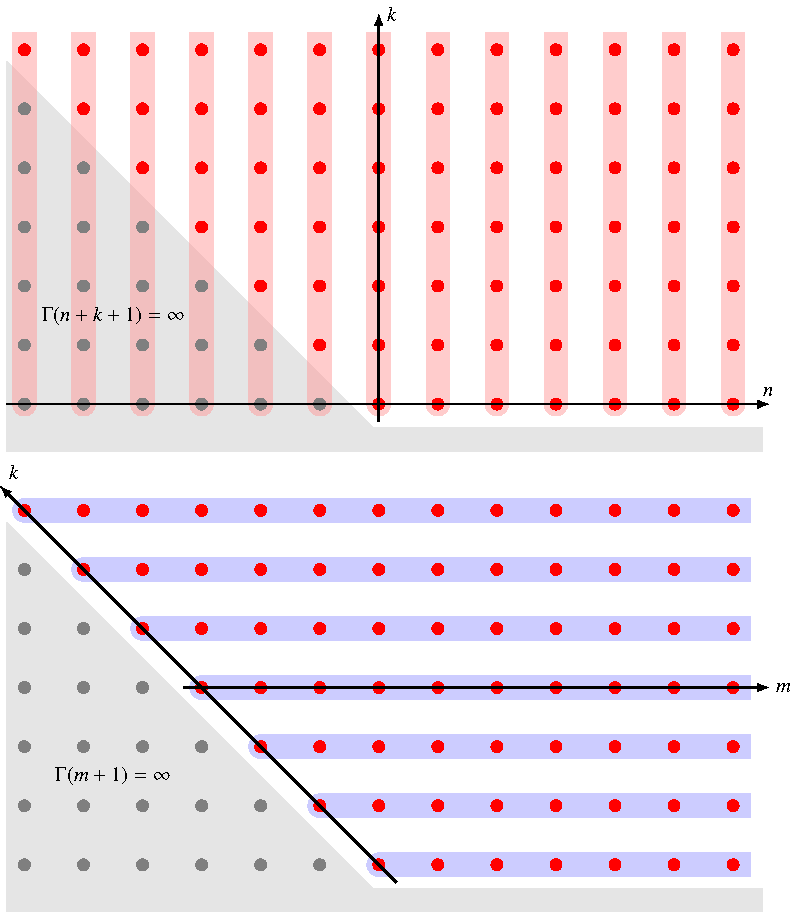
\includegraphics{chapters/050-differential/images/besselgrid.pdf}
\caption{Indexmenge für Herleitung der erzeugenden Funktion der
Besselfunktionen.
Die rote Summe in \eqref{buch:differentialgleichungen:bessel:eqn:rotesumme}
entspricht den vertikalen roten Streifen oben,
die blaue Summe in
\eqref{buch:differentialgleichungen:bessel:eqn:blauesumme}
den horizontalen Streifen in der Abbildung unten.
Alle Terme enthalten $\Gamma(n+k+1)$ im Nenner,
im grau hinterlegten Gebiet verschwinden sie.
\label{buch:differentialgleichungen:bessel:fig:indexmenge}}
\end{figure}
Die erzeugende Funktion der Bessel-Funktionen ist die Summe
\begin{align}
\sum_{n\in\mathbb{Z}} J_n(x)z^n
&=
\sum_{n\in\mathbb{Z}}
{\color{darkred}
\sum_{k=0}^\infty
\frac{(-1)^k}{k!\,\Gamma(k+n+1)}
\biggl(\frac{x}{2}\biggr)^{2k+n}
}
z^n.
\label{buch:differentialgleichungen:bessel:eqn:rotesumme}
\intertext{Die rote Summe entspricht den vertikalen roten Streifen in
Abbildung~\ref{buch:differentialgleichungen:bessel:fig:indexmenge} oben.
Die grau hinterlegten Punkte in der Abbildung gehören zu verschwindenden
Termen.
Wir schreiben $m=k+n$ und drücken alle Terme durch $k$ und $m$ aus:}
&=
\sum_{n\in \mathbb{Z}}
\sum_{k=0}^\infty
\frac{(-1)^k}{k!\,\Gamma(n+k+1)}
\biggl(\frac{x}{2}\biggr)^k
\biggl(\frac{x}{2}\biggr)^{n+k}
z^{n+k}
z^{-k}
\notag
\\
&=
\sum_{m\in \mathbb{Z}}
\sum_{k=0}^\infty \frac{(-1)^k}{k!}
\biggl(\frac{x}{2}\biggr)^k
z^{-k}
\frac{1}{\Gamma(m+1)}
\biggl(\frac{x}{2}\biggr)^{m}
z^{n+k}
\notag
\intertext{Auch in dieser Summe fallen wieder die Terme mit $m<0$
wegen $\Gamma(m+1)=\infty$ weg.
Die Grenzen der Summation über $k$ hängen nicht von $m$ ab, daher
können wir die Summationsreihenfolge vertauschen.
Die Summation über $m$ entspricht den horizontalen blauen Streifen
in 
Abbildung~\ref{buch:differentialgleichungen:bessel:fig:indexmenge}
unten.
Es ergibt sich die Summe}
&=
\sum_{k=0}^\infty
\sum_{m=0}^\infty
\frac{(-1)^k}{k!}
\biggl(\frac{x}{2}\biggr)^k
z^{-k}
\frac{1}{\Gamma(m+1)}
\biggl(\frac{x}{2}\biggr)^{m}
z^{m}
\notag
\\
&=
\sum_{k=0}^\infty \frac{(-1)^k}{k!}
\biggl(\frac{x}{2}\biggr)^k
z^{-k}
\cdot
{\color{blue}
\sum_{m=0}^\infty
\frac{1}{\Gamma(m+1)}
\biggl(\frac{x}{2}\biggr)^{m}
z^{m}
}.
\label{buch:differentialgleichungen:bessel:eqn:blauesumme}
\intertext{Beide Reihen sind Exponentialreihen, was man besser sehen kann,
wenn man die Gamma-Funktion in der zweiten Summe wieder als die
Fakultät $\Gamma(m+1)=m!$ schreibt.
Die beiden Exponentialreihen sind
}
&=
\sum_{k=0}^\infty \frac{\bigl(-\frac{x}2\cdot\frac1z\bigr)}{k!}
\cdot
\sum_{m=0}^\infty
\frac{\bigl(z\frac{x}2\bigr)^m}{m!}
=
\exp\biggl(\frac{x}2\cdot\biggl(-\frac1z\biggr)\biggr)
\cdot
\exp\biggl(\frac{x}2\cdot z\biggr)
=
\exp\biggl(\frac{x}2\cdot\biggl(z-\frac1z\biggr)\biggr).
\notag
\end{align}

%
% Additionstheorem
%
\subsubsection{Additionstheorem}
Die erzeugende Funktion kann dazu verwendet werden, das Additionstheorem
für die Besselfunktionen zu beweisen.

\begin{satz}
Für $l\in\mathbb{Z}$ und $x,y\in\mathbb{R}$ gilt
\[
J_l(x+y) = \sum_{m=-\infty}^\infty J_m(x)J_{l-m}(y).
\]
\end{satz}

\begin{proof}[Beweis]
Die Koeffizienten der erzeugenden Funktion der Bessel-Funktionen für
das Argument $x+y$ ist
\begin{align*}
\exp\biggl(\frac{x+y}2\biggl(z+\frac1z\biggr)\biggr)
&=
\sum_{n=-\infty}^\infty J_n(x+y)z^n.
\intertext{%
Wir verwenden die Exponentialgesetze auf der linken Seite und 
erhalten}
&=
\exp\biggl(\frac{x}2\biggl(z+\frac1z\biggr)\biggr)
\cdot
\exp\biggl(\frac{y}2\biggl(z+\frac1z\biggr)\biggr).
\intertext{Beide Faktoren sind erzeugende Funktionen von Bessel-Funktionen,
wir können sie also als}
&=
\sum_{m=-\infty}^\infty J_m(x)z^m
\cdot
\sum_{k=-\infty}^\infty J_k(y)z^k
\intertext{schreiben.
Durch Ausmultiplizieren und Zusammenfassen von Termen mit gleichem
Exponenten finden wir
}
&=
\sum_{m,k} J_m(x)J_k(y) z^{k+m}
=
\sum_{l=-\infty}^\infty
\biggl(
\sum_{m=-\infty}^\infty J_m(x)J_{l-m}(y)
\biggr)
z^l.
\intertext{Daraus folgt schliesslich mit Koeffizientenvergleich das
Additionstheorem}
J_l(x+y) &= \sum_{m=-\infty}^\infty J_m(x)J_{l-m}(y)
\end{align*}
für alle $l$.
\end{proof}

%
% Der Fall \alpha=0
% 
\subsubsection{Der Fall $\alpha=0$}
Im Fall $\alpha=0$ hat das Indexpolynom eine doppelte Nullstelle, wir
können daher nur eine Lösung erwarten.
Im Fall $\alpha=0$ wird das Produkt im Nenner zu $n!$, so dass die
Lösungsfunktion
\[
J_0(x)
=
\sum_{k=0}^\infty
\frac{(-1)^k}{(k!)^2}
\biggl(\frac{x}{2}\biggr)^{2k}
\]
geschrieben werden kann.


%
% Der Fall \alpha=p, p\in \mathbb{N}
%
\subsubsection{Der Fall $\alpha=p$, $p\in\mathbb{N}, p > 0$}
In diesem Fall kann nur die erste
Lösung~\eqref{buch:differentialgleichunge:bessel:erste}
verwendet werden.
Damit erhält die Lösungsfunktion die Form
\[
J_p(x)
=
\sum_{k=0}^\infty
\frac{(-1)^k}{k!(p+k)!}\biggl(\frac{x}{2}\biggr)^{p+2k}.
\]

%
% Der Fall $\alpha=n+\frac12$
%
\subsubsection{Der Fall $\alpha=n+\frac12$, $n\in\mathbb{N}$}
Obwohl $2\alpha$ eine Ganzzahl ist, sind die beiden Lösungen
\label{buch:differentialgleichunge:bessel:erste}
und
\label{buch:differentialgleichunge:bessel:zweite}
linear unabhängig.

Man kann zeigen, dass sich die Lösungsfunktionen in diesem Fall
durch bereits bekannte elementare Funktionen ausdrücken lassen.
Wir rechnen dies für $n=0$ nach.
Zunächst drücken wir die Pochhammer-Symbole im Nenner anders aus.
Es ist
\begin{align*}
\biggl(\frac12 + 1\biggr)_k
&=
\biggl(\frac12 + 1\biggr)
\biggl(\frac12 + 2\biggr)
\cdots
\biggl(\frac12 + k\biggr)
=
\frac{1}{2^k}\bigl(3\cdot 5\cdot\ldots\cdot (2k+1)\bigr)
=
\frac{(2k+1)!}{2^{2k}\cdot k!}
\\
\biggl(-\frac12 + 1\biggr)_k
&=
\biggl(-\frac12 + 1\biggr)
\biggl(-\frac12 + 2\biggr)
\cdots
\biggl(-\frac12 + k\biggr)
\\
&=
\biggl(\frac12 + 0\biggr)
\biggl(\frac12 + 1\biggr)
\cdots
\biggl(\frac12 + k-1\biggr)
=
\frac{1}{2^k}\bigl(1\cdot 3 \cdot\ldots\cdot (2(k-1)+1)\bigr)
=
\frac{(2k-1)!}{2^{2k-1}\cdot (k-1)!}
\end{align*}
Damit können jetzt die Reihenentwicklungen der Lösung wie folgt
umgeformt werden
\begin{align*}
y_1(x)
&=
x^\alpha
\sum_{k=0}^\infty
\frac{1}{(\alpha+1)_k}
\frac{(-x^2/4)^k}{k!}
=
\sqrt{x}
\sum_{k=0}^\infty
\frac{2^{2k}k!}{(2k+1)!}
\frac{(-x^2/4)^k}{k!}
=
\sqrt{x}
\sum_{k=0}^\infty
(-1)^k
\frac{x^{2k}}{(2k+1)!}
\\
&=
\frac{1}{\sqrt{x}}
\sum_{k=0}^\infty
(-1)^k
\frac{x^{2k+1}}{(2k+1)!}
=
\frac{1}{\sqrt{x}} \sin x
\\
y_2(x)
&=
x^{-\alpha}
\sum_{k=0}^\infty
\frac{1}{(-\alpha+1)_k}
\frac{(-x^2/4)^k}{k!}
=
x^{-\frac12}
\sum_{k=0}^\infty
\frac{2^{2k-1}\cdot (k-1)!}{(2k-1)!}
\frac{(-x^2/4)^k}{k!}
\\
&=
\frac{1}{\sqrt{x}}
\sum_{k=0}^\infty
(-1)^k
\frac{x^{2k}}{(2k-1)!\cdot 2k}
=
\frac{1}{\sqrt{x}} \cos x.
\end{align*}

Die Bessel-Funktionen verwenden aber eine andere Normierung. 
Die Gleichung~\eqref{buch:differentialgleichungen:bessel:normierungsgleichung}
zeigt, dass die Bessel-Funktionen durch Division
der Funktion $y_1(x)$ und $y_2(x)$ durch $2^\alpha \Gamma(\alpha+1)$ 
erhalten werden können.
Dies ergibt
\begin{equation*}
\renewcommand{\arraycolsep}{1pt}
\begin{array}{rclclclcl}
J_{\frac12}(x)
&=&
\displaystyle\frac{1}{2^{\frac12}\Gamma(\frac12+1)}
y_1(x)
&=&
\displaystyle\frac{1}{2^{\frac12}\frac12\Gamma(\frac12)}
y_1(x)
&=&
\displaystyle\frac{\sqrt{2}}{\Gamma(\frac12)}
y_1(x)
&=&
\displaystyle\frac{1}{\Gamma(\frac12)}
\sqrt{ \frac{2}{x}}
\sin x,
\\
J_{-\frac12}(x)
&=&
\displaystyle\frac{1}{2^{-\frac12}\Gamma(-\frac12+1)}
y_2(x)
&=&
\displaystyle\frac{2^{\frac12}}{\Gamma(\frac12)}
y_2(x)
&=&
\displaystyle\frac{\sqrt{2}}{\Gamma(\frac12)}
y_2(x)
&=&
\displaystyle\frac{1}{\Gamma(\frac12)}
\sqrt{\frac{2}{x}}
\cos x.
\end{array}
\end{equation*}
Wegen $\Gamma(\frac12)=\sqrt{\pi}$ sind die
halbzahligen Bessel-Funktionen daher
\begin{align*}
J_{\frac12}(x)
&=
\sqrt{\frac{2}{\pi x}} \sin x
=
\sqrt{\frac{2}{\pi}} x^{-\frac12}\sin x
&
&\text{und}&
J_{-\frac12}(x)
&=
\sqrt{\frac{2}{\pi x}} \cos x
=
\sqrt{\frac{2}{\pi}} x^{-\frac12}\cos x.
\end{align*}

%
% Direkte Verifikation der Lösungen
%
\subsubsection{Direkte Verifikation der Lösungen für $\alpha=\pm\frac12$}
Tatsächlich führt die Anwendung des Bessel-Operators auf die beiden
Funktionen auf
\begin{align*}
\sqrt{\frac{\pi}2}
BJ_{\frac12}(x)
&=
\sqrt{\frac{\pi}2}
\biggl(
x^2J_{\frac12}''(x) + xJ_{\frac12}'(x) + x^2J_{\frac12}(x)
\biggr)
\\
&=
x^2(x^{-\frac12}\sin x)''
+
x(x^{-\frac12}\sin x)'
+
x^2(x^{-\frac12}\sin x)
\\
&=
x^2(
x^{-{\textstyle\frac12}}\cos x
-{\textstyle\frac12}x^{-\frac32}\sin x
)'
+
x(
x^{-\frac12}\cos x
-{\textstyle\frac12}x^{-\frac32}\sin x
)
+
x^{\frac32}\sin x
\\
&=
x^2(
-x^{-\frac12}\sin x
-{\textstyle\frac12}x^{-\frac32}\cos x
-{\textstyle\frac12}x^{-\frac32}\cos x
+{\textstyle\frac{3}{4}}x^{-\frac52}\sin x
)
+
x^{\frac12}\cos x
+
x^{-\frac12}(x-{\textstyle\frac12})\sin x
\\
&=
(
-x^{\frac32}
+{\textstyle\frac34}x^{-\frac12}
+x^{\frac32}
-{\textstyle\frac12}x^{-\frac12}
)
\sin x
=
\frac14x^{-\frac12}\sin x
=
\frac14
\sqrt{\frac{\pi}2}
J_{\frac12}(x)
\\
BJ_{\frac12}(x)
&=
\biggl(\frac12\biggr)^2 J_{\frac12}(x).
\end{align*}
Dies zeigt, dass $J_{\frac12}(x)$ tatsächlich eine Eigenfunktion
des Bessel-Operators zum Eigenwert $\alpha^2 = \frac14$ ist.
Analog kann man die Lösung $y_2(x)$ für $-\frac12$ verifizieren.


%
% sturm.tex
%
% (c) 2022 Prof Dr Andreas Müller, OST Ostschweizer Fachhochschule
%
\section{Das Sturm-Liouville-Problem
\label{buch:integrale:subsection:sturm-liouville-problem}}
\rhead{Das Sturm-Liouville-Problem}
Sowohl bei den Bessel-Funktionen wie bei den Legendre-Polynomen
\index{Bessel-Funktion}%
konnte die Orthogonalität der Funktionen dadurch gezeigt werden,
dass sie als Eigenfunktionen eines bezüglich eines geeigneten
Skalarproduktes selbstadjungierten Operators erkannt wurden.

%
% Differentialgleichungen
%
\subsection{Differentialgleichung}
Das klassische Sturm-Liouville-Problem ist das folgende Eigenwertproblem.
Gesucht sind Lösungen der Differentialgleichung
\begin{equation}
((p(x)y'(x))' + q(x)y(x) = \lambda w(x) y(x)
\label{buch:integrale:eqn:sturm-liouville}
\end{equation}
auf dem Intervall $(a,b)$, die zusätzlich die Randbedingungen
\begin{equation}
\begin{aligned}
k_a y(a) + h_a p(a) y'(a) &= 0 \\
k_b y(b) + h_b p(b) y'(b) &= 0
\end{aligned}
\label{buch:integrale:sturm:randbedingung}
\end{equation}
erfüllen, wobei $|k_i|^2 + |h_i|^2\ne 0$ mit $i=a,b$.
Weitere Bedingungen an die Funktionen $p(x)$, $q(x)$, $w(x)$  sowie die
Lösungsfunktionen $y(x)$ sollen später geklärt werden.

%
% Das verallgemeinerte Eigenwertproblem für symmetrische Matrizen
%
\subsection{Das verallgemeinerte Eigenwertproblem für symmetrische Matrizen}
Ein zu \eqref{buch:integrale:eqn:sturm-liouville} analoges Eigenwertproblem
für Matrizen ist das folgende verallgemeinerte Eigenwertproblem.
Das gewohnte Eigenwertproblem verwendet die Matrix $B=E$.

\begin{definition}
\index{verallgemeinerter Eigenvektor}%
\index{Eigenvektor, verallgemeinerter}%
\label{buch:orthogonal:sturm:verallgemeinerter-eigenvektor}
Seien $A$ und $B$ $n\times n$-Matrizen.
$v$ heisst {\em verallgemeinerter Eigenvektor} zum Eigenwert $\lambda$,
wenn
\[
Av = \lambda Bv.
\]
\end{definition}

Für symmetrische Matrizen lässt sich dieses Problem auf ein 
Optimierungsproblem reduzieren.

\begin{satz}
\index{Satz!verallgemeinertes Eigenwertproblem}%
Seien $A$ und $B$ symmetrische $n\times n$-Matrizen und sei ausserdem
$B$ positiv definit.
Ist $v$ ein Vektor, der die Grösse
\[
f(v)=\frac{v^tAv}{v^tBv}
\]
maximiert, ist ein verallgemeinerter Eigenvektor für die Matrizen $A$
und $B$.
\end{satz}

\begin{proof}[Beweis]
Sei $\lambda = f(v)$ der maximale Wert und $u\ne 0$ ein beliebiger Vektor. 
Da $v$ die Grösse $f(v)$ maximiert, muss die Ableitung
von $f(u+tv)$ für $t=0$ verschwinden.
Um diese Ableitung zu berechnen, bestimmen wir zunächst die Ableitung
von $(v+tu)^tM(v+tu)$  an der Stelle $t=0$ für eine beliebige
symmetrische Matrix:
\begin{align*}
\frac{d}{dt}
(v+tu)^tM(v+tu)
&=
\frac{d}{dt}\bigl(
v^tv + t(v^tMu+u^tMv) + t^2 u^tMu
\bigr)
=
v^tMu+u^tMv + 2tv^tMv
\\
\frac{d}{dt}
(v^t+tu^t)M(v+tu)
\bigg|_{t=0}
&=
v^tMu+u^tMv
=
2v^tMu
\end{align*}
Dies wenden wir jetzt auf den Quotenten $\lambda(v+tu)$ an.
\begin{align*}
\frac{d}{dt}f(v+tu)\bigg|_{t=0}
&=
\frac{d}{dt}
\frac{(v+tu)^tA(v+tu)}{(v+tu)^tB(v+tu)}\bigg|_{t=0}
\\
&=
\frac{2u^tAv(v^tBv) - 2u^tBv(v^tAv)}{(v^tBv)^2}
=
\frac{2}{v^tBv}
u^t
\biggl(
Av - \frac{v^tAv}{v^tBv} Bv
\biggr)
\\
&=
2
\frac{
u^t(
Av - \lambda Bv
)
}{v^tBv}
\end{align*}
Da $v$ ein Maximum von $\lambda(v)$ ist, verschwindet diese Ableitung
für alle Vektoren $u$, somit gilt
\[
u^t(Av-\lambda Bv)=0
\]
für alle $u$, also auch $Av=\lambda Bv$.
Dies beweist, dass $v$ ein verallgemeinerter Eigenvektor zum
Eigenwert $\lambda$ ist.
\end{proof}

\begin{satz}
\index{Satz!Orthogonalität verallgemeinerter Eigenvektoren}%
Verallgemeinerte Eigenvektoren $u$ und $v$ von $A$ und $B$
zu verschiedenen Eigenwerten erfüllen $u^tBv=0$.
\end{satz}

\begin{proof}
Seien $\lambda$ und $\mu$ die Eigenwerte, also $Au=\lambda Bu$
und $Av=\mu Bv$.
Wie in \eqref{buch:integrale:eqn:eigenwertesenkrecht}
berechnen wir das Skalarprodukt auf zwei Arten
\[
\renewcommand{\arraycolsep}{2pt}
\begin{array}{rcccrl}
 u^tAv &=&u^t\lambda Bv &=& \lambda\phantom{\mathstrut-\mu)} u^tBv
	&\multirow{2}{*}{\hspace{3pt}$\bigg\}\mathstrut-\mathstrut$}\\
=v^tAu &=&v^t\mu Bu     &=&  \mu\phantom{)}u^tBv         &\\
\hline
     0 & &              &=& (\lambda - \mu)u^tBv.        &
\end{array}
\]
Da die Eigenwerte verschieden sind, ist $\lambda-\mu\ne 0$, es folgt, 
dass $u^tBv=0$ sein muss.
\end{proof}

Verallgemeinerte Eigenwerte und Eigenvektoren verhalten sich also
ganz analog zu den gewöhnlichen Eigenwerten und Eigenvektoren.
Da $B$ positiv definit ist, ist $B$ auch invertierbar.
\index{verallgemeinertes Skalarprodukt}%
\index{Skalarprodukt!verallgemeinertes}%
Zudem kann $B$ zur Definition des verallgemeinerten Skalarproduktes
\[
\langle u,v\rangle_B = u^tBv
\]
verwendet werden.
Die Matrix 
\[
\tilde{A} = B^{-1}A
\]
ist bezüglich dieses Skalarproduktes selbstadjungiert, denn es gilt
\[
\langle\tilde{A}u,v\rangle_B
=
(B^{-1}Au)^t Bv
=
u^tA^t(B^{-1})^tBv
=
u^tAv
=
u^tBB^{-1}Av
=
\langle u,\tilde{A}v\rangle.
\]
Das verallgemeinerte Eigenwertproblem für symmetrische Matrizen
ist damit ein gewöhnliches Eigenwertproblem für selbstadjungierte
Matrizen des Operators $\tilde{A}$ bezüglich des verallgemeinerten
Skalarproduktes $\langle\,\;,\;\rangle_B$.

%
% Der Operator L_0 und die Randbedingung
%
\subsection{Der Operator $L_0$ und die Randbedingung}
Die Differentialgleichung kann auch in Operatorform geschrieben werden.
Dazu schreiben wir
\[
L_0 
=
-\frac{d}{dx}p(x)\frac{d}{dx}.
\]
Bezüglich des gewöhnlichen Skalarproduktes
\[
\langle f,g\rangle
=
\int_a^b f(x)g(x)\,dx
\]
für Funktionen auf dem Intervall $[a,b]$ ist der Operator $L_0$
tatsächlich selbstadjungiert.
Mit partieller Integration rechnet man nach:
\index{partielle Integration}%
\begin{align}
\langle f,L_0g\rangle
&=
\int_a^b f(x) \biggl(-\frac{d}{dx}p(x)\frac{d}{dx}\biggr)g(x)\,dx
\notag
\\
&=
-\int_a^b f(x) \frac{d}{dx}\bigl( p(x) g'(x) \bigr)\,dx
\notag
\\
&=
-\biggl[f(x) p(x)g'(x)\biggr]_a^b
+
\int_a^b f'(x) p(x) g'(x) \,dx
\notag
\\
\langle L_0f,g\rangle
&=
-\biggl[f'(x)p(x)g(x)\biggr]_a^b
+
\int_a^b f'(x) p(x) g'(x) \,dx.
\notag
\intertext{Die beiden Skalarprodukte führen also auf das gleiche
Integral, sie unterscheiden sich nur um die Randterme}
\langle f,L_0g\rangle
-
\langle L_0f,g\rangle
&=
-f(b)p(b)g'(b) + f(a)p(a)g'(a)
+f'(b)p(b)g(b) - f'(a)p(a)g(a)
\label{buch:integrale:sturm:sabedingung}
\\
&=
-
p(b)
\left|\begin{matrix}
f(b) &g(b)\\
f'(b)&g'(b)
\end{matrix}\right|
+
p(a)
\left|\begin{matrix}
f(a) &g(a)\\
f'(a)&g'(a)
\end{matrix}\right|
\notag
\\
&=
-
\left|\begin{matrix}
f(b) &g(b)\\
p(b)f'(b)&p(b)g'(b)
\end{matrix}\right|
+
\left|\begin{matrix}
f(a) &g(a)\\
p(a)f'(a)&p(a)g'(a)
\end{matrix}\right|.
\notag
\end{align}
Um zu erreichen, dass der Operator selbstadjunigert wird, muss 
sichergestellt werden, dass entweder $p$ oder die Determinanten
an den Intervallenden verschwinden.
Dies passiert genau dann, wenn die Vektoren 
\[
\begin{pmatrix}
f(a)\\
p(a)f'(a)
\end{pmatrix}
\text{\;und\;}
\begin{pmatrix}
g(a)\\
p(a)g'(a)
\end{pmatrix}
\]
linear abhängig sind.
In zwei Dimensionen bedeutet lineare Abhängigkeit, dass es
eine nichttriviale Linearform mit Koeffizienten $h_a, k_a$ gibt,
die auf beiden Vektoren verschwindet.
Ausgeschrieben bedeutet dies, dass die Randbedingung
\eqref{buch:integrale:sturm:randbedingung}
erfüllt sein muss.

%
% Skalarprodukt
%
\subsection{Skalarprodukt}
Das Ziel der folgenden Abschnitte ist, das Sturm-Liouville-Problem als
Eigenwertproblem für einen selbstadjungierten Operator in einem 
Funktionenraum mit einem geeigneten Skalarprodukt zu finden.

Wir haben bereits gezeigt, dass die Randbedingung
\eqref{buch:integrale:sturm:randbedingung} sicherstellt, dass der
Operator $L_0$ für das Standardskalarprodukt selbstadjungiert ist.
Dies entspricht der Symmetrie der Matrix $A$.

Die Komponente $q(x)$ stellt keine besonderen Probleme, denn
\[
\langle f,qg\rangle
=
\int_a^b f(x)q(x)g(x)\,dx
=
\langle qf,g\rangle.
\]
Der Operator $f(x) \mapsto q(x)f(x)$, der eine Funktion mit 
der Funktion $q(x)$ multipliziert, ist also ebenfalls symmetrisch.
Dasselbe gilt für einen Operator, der mit $w(x)$ multipliziert.
Da $w(x)$ eine positive Funktion ist, ist der Operator $f(x)\mapsto w(x)f(x)$
sogar positiv definit.
Dies entspricht der Matrix $B$.
Nach den Erkenntnissen des vorangegangenen Abschnittes ist das
verallgemeinerte Eigenwertproblem daher ein Eigenwertproblem
für einen modifizierten Operator bezüglich eines alternativen
Skalarproduktes.

Als Skalarprodukt muss also das Integral
\[
\langle f,g\rangle_w
=
\int_a^b f(x)g(x)w(x)\,dx
\]
mit der Gewichtsfunktion $w(x)$ verwendet werden.
Damit dies ein vernünftiges Skalarprodukt ist, muss $w(x)>0$ im
Innerend es Intervalls sein.

%
% Der Vektorraum H
%
\subsection{Der Vektorraum $H$}
Damit können wir jetzt die Eigenschaften der in Frage kommenden
Funktionen zusammenstellen.
Zunächst müssen sie auf dem Intervall $[a,b]$ definiert sein und
das Integral
\[
\int_a^b |f(x)|^2 w(x)\,dx < \infty
\]
muss existieren.
Wir bezeichnen den Vektorraum der Funktionen, deren Quadrat mit
der Gewichtsfunktion $w(x)$ integrierbar sind, mit
$L^2([a,b],w)$.

Damit auch $\langle qf,f\rangle_w$ und $\langle L_0f,f\rangle_w$
wohldefiniert sind, müssen zusätzlich die Integrale
\[
\int_a^b |f(x)|^2 q(x) w(x)\,dx
\qquad\text{und}\qquad
\int_a^b |f'(x)|^2 p(x) w(x)\,dx
\]
existieren.
Wir setzen daher
\[
H
=
\biggl\{
f\in L^2([a,b],w)\;\bigg|\;
\int_a^b |f'(x)|^2p(x)w(x)\,dx<\infty,
\int_a^b |f(x)|^2q(x)w(x)\,dx<\infty
\biggr\}.
\]

%
% Der Sturm-Liouville-Differentialoperator
%
\subsection{Der Sturm-Liouville-Differentialoperator}
Das verallgemeinerte Eigenwertproblem für $A$ und $B$ ist ein
gewöhnliches Eigenwertproblem für die Operator $\tilde{A}=B^{-1}A$
bezüglich des modifizierten Skalarproduktes.
Das Sturm-Liouville-Problem ist also ein Eigenwertproblem im
Vektorraum $H$ mit dem Skalarprodukt $\langle\,\;,\;\rangle_w$.
Der Operator
\begin{equation}
L = \frac{1}{w(x)} \biggl(-\frac{d}{dx} p(x)\frac{d}{dx} + q(x)\biggr)
\label{buch:orthogonal:sturm-liouville:opL1}
\end{equation}
heisst der {\em Sturm-Liouville-Operator}.
\index{Sturm-Liouville-Operator}%
\index{Operator!Sturm-Liouville-}%
Eine Lösung des Sturm-Liouville-Problems ist eine Funktion $y(x)$ derart,
dass 
\[
Ly = \lambda y,
\]
$\lambda$ ist der zu $y(x)$ gehörige Eigenwert.
Der Operator ist definiert auf Funktionen des im vorangegangenen Abschnitt
definierten Vektorraumes $H$.
Führt man die Differentiation aus, bekommt der Operator die Form
\begin{equation}
L
=
-\frac{p(x)}{w(x)} \frac{d^2}{dx^2}
-\frac{p'(x)}{w(x)} \frac{d}{dx}
+\frac{q(x)}{w(x)}.
\label{buch:orthogonal:sturm-liouville:opL2}
\end{equation}

%
% Beispiele
%
\subsection{Beispiele}
Die meisten der früher vorgestellten Funktionenfamilien stellen sich
als Lösungen eines geeigneten Sturm-Liouville-Problems heraus.
Alle Eigenschaften aus der Sturm-Liouville-Theorie gelten daher
automatisch für diese Funktionenfamilien.

%
% Trignometrische Funktionen
%
\subsubsection{Trigonometrische Funktionen}
Die trigonometrischen Funktionen sind Eigenfunktionen des Operators
$d^2/dx^2$, also eines Sturm-Liouville-Operators mit $p(x)=1$, $q(x)=0$
und $w(x)=1$.
Auf dem Intervall $(-\pi,\pi)$ können wir die Randbedingungen
\bgroup
\renewcommand{\arraycolsep}{2pt}
\[
\begin{aligned}
&
\begin{array}{lclclcl}
k_{-\pi}          &=&1,&\qquad&h_{-\pi}          &=&0\\
k_{\phantom{-}\pi}&=&1,&\qquad&h_{\phantom{-}\pi}&=&0
\end{array}
\;\bigg\}
&&\Rightarrow&
\begin{array}{lcl}
y(-\pi)          &=&0\\
y(\phantom{-}\pi)&=&0\\
\end{array}
\;\bigg\}
&\quad\Rightarrow&
y(x) &= B\sin nx
\\
&
\begin{array}{lclclcl}
k_{-\pi}          &=&0,&\qquad&h_{-\pi}          &=&1\\
k_{\phantom{-}\pi}&=&0,&\qquad&h_{\phantom{-}\pi}&=&1
\end{array}
\;\bigg\}
&&\Rightarrow&
\begin{array}{lcl}
y'(-\pi)          &=&0\\
y'(\phantom{-}\pi)&=&0\\
\end{array}
\; \bigg\}
&\quad\Rightarrow&
y(x) &= A\cos nx
\end{aligned}
\]
\egroup
verwenden.
Die Orthogonalität der Sinus- und Kosinus-Funktionen folgt jetzt
ganz ohne weitere Rechnung.

An dieser Lösung ist nicht ganz befriedigend, dass die trigonometrischen
Funktionen nicht mit einer einzigen Randbedingung gefunden werden können.
Der Ausweg ist, periodische Randbedingungen zu verlangen, also
$y(-\pi)=y(\pi)$ und $y'(-\pi)=y'(\pi)$.
Dann ist wegen
\begin{align*}
\langle f,L_0g\rangle - \langle L_0f,g\rangle
&=
-f(\pi)g'(\pi)+f(-\pi)g'(-\pi)+f'(\pi)g(\pi)-f'(-\pi)g(-\pi)
\\
&=
-f(\pi)g'(\pi)+f(\pi)g'(\pi)+f'(\pi)g(\pi)-f'(\pi)g(\pi)
=0
\end{align*}
die Bedingung~\eqref{buch:integrale:sturm:sabedingung}
ebenfalls erfüllt, $L_0$ ist in diesem Raum selbstadjungiert.

%
% Bessel-Funktionen J_n(x)
%
\subsubsection{Bessel-Funktionen $J_n(x)$}
Der Bessel-Operator \eqref{buch:differentialgleichungen:bessel-operator}
kann wie folgt in die Form eines Sturm-Liouville-Operators gebracht 
werden.
Zunächst rechnet man
\[
B
=
x^2\frac{d^2}{dx^2} + x\frac{d}{dx} + x^2
=
x\biggl(
x\frac{d^2}{dx^2} + \frac{d}{dx} + x
\biggr)
=
x\biggl(
\frac{d}{dx}(-x)\frac{d}{dx} + x
\biggr).
\]
Somit ist $B$ ein Sturm-Liouville-Operator für 
\begin{equation}
\begin{aligned}
p(x) &= -x \\
q(x) &= x \\
w(x) &= \frac{1}{x}.
\end{aligned}
\label{buch:orthogonal:sturm:bessel:n}
\end{equation}
Am linken Rand kann als Randbedingung 
\[
\lim_{x\to 0} p(x) y'(x) = 0
\]
verwendet werden, die für alle Bessel-Funktionen erfüllt ist.
Dies entspricht der Wahl $k_0=0$ und $h_0=1$.
Am rechten Rand für $x\to\infty$ kann man
\[
\lim_{x\to\infty} y(x)=0
\]
verlangen, was der Wahl $k_\infty=1$ und $h_\infty=0$ entspricht.
Damit ist die Bessel-Differentialgleichung erkannt als ein
Sturm-Liouville-Problem für $\lambda=n^2$.
Es folgt damit sofort, dass die Besselfunktionen orthogonale
Funktionen bezüglich des Skalarproduktes mit der Gewichtsfunktion
$w(x)=1/x$ sind.

%
% Bessel-Funktionen J_n(sx)
%
\subsubsection{Bessel-Funktionen $J_n(s x)$}
Das Sturm-Liouville-Problem mit den Funktionen
\eqref{buch:orthogonal:sturm:bessel:n}
ist jedoch nicht die einzige Möglichkeit, die Bessel-Differentialgleichung
in ein Sturm-Liouville-Problem zu verwandeln.
Das Problem \eqref{buch:orthogonal:sturm:bessel:n} ging davon
aus, dass $n^2$ der verallgemeinerte Eigenwert sein soll.
Im Folgenden sollen hingegen die Funktionen $J_n(s x)$ für
konstantes $n$, aber verschiedene $s$ untersucht und
als orthogonal erkannt werden.

Die Funktion $y(x) = J_n(x)$ ist eine Lösung der Besselschen
Differentialgleichung
\index{Besselsche Differentialgleichung}%
\index{Differentialgleichung!Besselsche}%
\[
x^2y'' + xy' + x^2y = n^2y.
\]
Setzt man $x=s t$ und $f(t)=y(s t)$, dann wird die Ableitung 
\[
\begin{aligned}
f'(t)
&=
\frac{d}{dt}y(s t)
=
y'(s t) \cdot s
&&\Rightarrow
&
\frac{f'(t)}{s}
&=
y'(x)
\\
f''(t)
&=
\frac{d^2}{dt^2} y(s t)
=
y''(s t) \cdot s^2
&&\Rightarrow
&
\frac{f''(t)}{s^2}
&=
y''(x).
\end{aligned}
\]
Setzt man diese in die Besselsche Differentialgleichung ein,
findet man
\begin{align*}
x^2y''+xy'+x^2y
=
s^2 t^2 \frac{f''(t)}{s^2}
+
s t \frac{f'(t)}{s}
+
s^2 t^2 f(t)
&=
n^2 f(t).
\end{align*}
Damit ist gezeigt, dass die Funktionen $J_n(s x)$ Lösungen
der Differentialgleichung
\begin{equation}
x^2y'' + xy' + (s^2 x^2  - n^2) y = 0
\label{buch:orthogonal:sturm:eqn:bessellambda}
\end{equation}
ist.

Die Differentialgleichung
\eqref{buch:orthogonal:sturm:eqn:bessellambda}
soll jetzt ebenfalls als ein Sturm-Liouville-Problem betrachtet
werden, diesmal aber mit festem $n$ und $s^2$ als dem verallgemeinerten
Eigenwert.
Dazu wird
\begin{equation}
\begin{aligned}
p(x) &= -x \\
q(x) &= -\frac{n^2}{x} \\
w(x) &= x
\end{aligned}
\label{buch:orthgonal:sturm:bessel:lambdaparams}
\end{equation}
gesetzt.
Das zugehörige Sturm-Liouville-Problem ist jetzt
\[
\frac{1}{x}\biggl(
\frac{d}{dx} (-x)\frac{d}{dx} -\frac{n^2}{x}
\biggr)
y
=
\lambda y
\quad\Rightarrow\quad
y'' + \frac{1}{x}y' - \frac{n^2}{x^2}y = \lambda y,
\]
oder nach Multiplikation mit $x^2$
\begin{equation}
x^2y'' + xy' + ((-\lambda)x^2 - n^2) y = 0.
\end{equation}
Die Funktionen $J_n(sx)$ sind daher verallgemeinerte Eigenfunktionen
des Sturm-Liouville-Problems
\eqref{buch:orthgonal:sturm:bessel:lambdaparams}
für den Eigenwert $\lambda = -s^2$.

\begin{satz}[Orthogonalität der Bessel-Funktionen]
\index{Satz!Orthogonalität der Bessel-Funktionen}%
Die Bessel-Funktionen $J_n(sx)$ für verschiedene $s$ sind orthogonal
bezüglich des Skalarproduktes mit der Gewichtsfunktion $w(x)=x$,
d.~h.
\[
\int_0^\infty J_n(s_1x) J_n(s_2x) x\,dx
=
0
\]
für $s_1\ne s_2$.
\end{satz}

\begin{proof}[Beweis]
Um die Bessel-Funktionen als Lösung des Sturm-Liouville-Problems
\eqref{buch:orthgonal:sturm:bessel:lambdaparams}
zu betrachten, müssen noch geeignete Randbedingungen formuliert werden.
Für $n>0$ kann man 
$J_n(0)=0$ verwenden, also $k_0=1$ und $h_0=0$.
Für $J_0$ ist dies nicht geeignet, aber wegen $J_0'(0)=0$ kann
man für $n=0$ verwenden $k_0=0$ und $h_0=1$ wählen.

Für den rechten Rand kann man verwenden, dass die Ableitung der
Bessel-Funktionen wie $x^{-3/2}$ gegen $0$ geht, gilt
\[
\lim_{x\to\infty} p(x) J_n(sx) = 0,
\]
weil $p(x)J_n(sx)$ wie $x^{-1/2}$ gegen $0$ geht.
Dies bedeutet, dass $k_\infty=0$ und $h_\infty=1$
verwendet werden kann.
Damit sind geeignete Randbedingungen für das Sturm-Liouville-Problem
gefunden.
\end{proof}

%
% Laguerre-Polynome
%
\subsubsection{Laguerre-Polynome}
Die Laguerre-Polynome sind orthogonal bezüglich des Skalarprodukts
mit der Laguerre-Gewichtsfunktion $w(x)=e^{-x}$ und erfüllen die
Laguerre-Differentialgleichung
\eqref{buch:differentialgleichungen:eqn:laguerre-dgl}.
mit $p(x)=-xe^{-x}$ wird 
\[
\frac{1}{w(x)}
\biggl(
-
\frac{d}{dx} p(x) \frac{d}{dx}
\biggr)
=
e^x \biggl(xe^{-x}\frac{d^2}{dx^2} + (1-x)e^{-x}\frac{d}{dx}\biggr),
\]
dies sind die abgeleiteten Terme in der Laguerre-Differentialgleichung.
Der Definitionsbereich ist $(0,\infty)$.
Als Randbedingung am linken kann man $y(0)=1$ verwenden, welche
auch die Laguerre-Polynome ergeben hat.
Am rechten Rand ist die Bedingung
\[
\lim_{x\to\infty} p(x)y'(x)
=
\lim_{x\to\infty} xe^{-x} y'(x)
=
0
\]
für beliebige Polynomlösungen erfüllt, dies ist der Fall
$k_{\infty}=0$ und $h_\infty=1$.

Das zugehörige verallgemeinerte Eigenwertproblem  wird damit
\[
xy'' + (1-x)y' - \lambda y = 0,
\]
also die Laguerre-Differentialgleichung.
Somit folgt, dass die Laguerre-Polynome orthogonal sind bezüglich
des Skalarproduktes mit der Laguerre-Gewichtsfunktion.

%
% Tschebyscheff-Polynome
%
\subsubsection{Tschebyscheff-Polynome}
Die Tschebyscheff-Polynome sind Lösungen der
bereits in Kapitel~\ref{buch:chapter:potenzen} hergeleiteten
Tschebyscheff-Differentialgleichung~\eqref{buch:potenzen:tschebyscheff:dgl}
\index{Tschebyscheff-Differentialgleichung}%
\index{Differentialgleichung!Tschebyscheff-}%
\[
(1-x^2)y'' -xy' = n^2y
\]
auf dem Intervall $(-1,1)$.
Auch dieses Problem kann als Sturm-Liouville-Problem formuliert
werden mit
\begin{align*}
w(x) &= \frac{1}{\sqrt{1-x^2}} \\
p(x) &= \sqrt{1-x^2} \\
q(x) &= 0
\end{align*}
Das zugehörige Sturm-Liouville-Eigenwertproblem ist
\[
\frac{d}{dx}\sqrt{1-x^2}\frac{d}{dx} y(x)
=
\lambda \frac{1}{\sqrt{1-x^2}} y(x).
\]
Führt man die Ableitungen auf der linken Seite aus, entsteht die
Gleichung
\begin{align*}
\sqrt{1-x^2} y''(x) -\frac{x}{\sqrt{1-x^2}}y'(x)
&=  \lambda \frac{1}{\sqrt{1-x^2}} y(x)
\intertext{Multiplikation mit $\sqrt{1-x^2}$ ergibt}
(1-x^2)
y''(x) 
-
xy'(x)
&=
\lambda y(x).
\end{align*}
Es folgt, dass die Tschebyscheff-Polynome orthogonal sind 
\index{Tschebyscheff-Polynom}%
bezüglich des Skalarproduktes
\[
\langle f,g\rangle = \int_{-1}^1 f(x)g(x)\frac{dx}{\sqrt{1-x^2}}.
\]

%
% Jacobi-Polynome
%
\subsubsection{Jacobi-Polynome}
Die Jacobi-Polynome sind orthogonal bezüglich des Skalarproduktes
\index{Jacobi-Polynome}%
\index{Polynome!Jacobi-}%
mit der Gewichtsfunktion
\[
w^{(\alpha,\beta)}(x) = (1-x)^\alpha(1+x)^\beta,
\]
definiert in Definition~\ref{buch:orthogonal:def:jacobi-gewichtsfunktion}.
%Bei der Herleitung der Rodrigues-Formel für die Jacobi-Polynome wurde erkannt,
%dass $B(x)=1-x^2$ und $A(x)=\beta-\alpha-(\alpha+\beta)x$ sein muss.
Man kann zeigen, dass sie Lösungen der
{\em Jacobi-Diffe\-ren\-tial\-gleichung}
\index{Jacobi-Differentialgleichung}%
\index{Differentialgleichung!Jacobi}%
\begin{equation}
(1-x^2)y'' + (\beta-\alpha-(\alpha+\beta + 2)x)y' + n(n+\alpha+\beta+1)y=0
\label{buch:orthogonal:jacobi:dgl}
\end{equation}
sind.
Es stellt sich die Frage, ob sich Funktionen $p(x)$ und $q(x)$ finden lassen
derart, dass die Differentialgleichung~\eqref{buch:orthogonal:jacobi:dgl}
eine Sturm-Liouville-Gleichung wird.
Gemäss der Form~\eqref{buch:orthogonal:sturm-liouville:opL2} muss
$p(x)$ so gefunden werden, dass
\begin{align*}
\frac{p(x)}{w^{(\alpha,\beta)}(x)} &= 1-x^2 \\
\frac{p'(x)}{w^{(\alpha,\beta)}(x)} &= \beta-\alpha-(\alpha+\beta+2)x
\end{align*}
gilt.
Der Quotient der beiden Gleichungen ist die logarithmische Ableitung
\[
(\log p(x))'
=
\frac{p'(x)}{p(x)}
=
\frac{1-x^2}{\beta-\alpha-(\alpha+\beta+2)x}
\]
von $p(x)$,
die sich in geschlossener Form integrieren lässt.
Man findet als Stammfunktion
\[
p(x)
=
(1-x)^{\alpha+1}(1+x)^{\beta+1}.
\]
Tatsächlich ist
\begin{align*}
\frac{p(x)}{w^{(\alpha,\beta)}(x)}
&=
\frac{(1-x)^{\alpha+1}(1+x)^{\beta+1}}{(1-x)^\alpha(1+x)^\beta}
=
(1-x)(1+x)=1-x^2
\\
\frac{p'(x)}{w^{(\alpha,\beta)}(x)}
&=
\frac{
-(\alpha+1)
(1-x)^{\alpha}(1+x)^{\beta+1}
+
(\beta+1)
(1-x)^{\alpha+1}(1+x)^{\beta}
}{
(1-x)^{\alpha}(1+x)^{\beta}
}
\\
&=
-(\alpha+1)(1+x) + (\beta+1)(1-x)
=
\beta-\alpha-(\alpha+\beta+2)x.
\end{align*}
Damit ist
die Jacobische Differentialgleichung 
als Sturm-Liouville-Differentialgleichung erkannt.

%
% Hypergeometrische Differentialgleichungen
%
\subsubsection{Hypergeometrische Differentialgleichungen}
%\url{https://encyclopediaofmath.org/wiki/Hypergeometric_equation}
Auch die Eulersche hypergeometrische Differentialgleichung
\index{Eulersche hypergeometrische Differentialgleichung}%
\index{Differentialgleichung!Eulersche hypergeometrische}%
lässt sich in die Form eines Sturm-Liouville-Operators
\index{Eulersche hypergeometrische Differentialgleichung!als Sturm-Liouville-Gleichung}%
bringen.
Dazu setzt man
\begin{align*}
p(z)
&=
z^c(z-1)^{a+b+1-c}
\\
q(z)
&=
-abz^{c-1}(z-1)^{a+b-c}
\\
w(z)
&=
z^{c-1}(z-1)^{a+b-c}.
\end{align*}
Setzt man dies in den Sturm-Liouville-Operator ein, erhält man
\begin{equation}
L
=
-\frac{d}{dz}p(z)\frac{d}{dz} + q(z)
=
-p(z)\frac{d^2}{dz^2}
-p'(z)\frac{d}{dz}
+q(z)
\label{buch:orthgonalitaet:eqn:hypersturm}
\end{equation}
Wir brauchen also
\begin{align*}
p'(z)
&=
cz^{c-1}(z-1)^{a+b+1-c}
+
(a+b+1-c)
z^c
(z-1)^{a+b-c}
\\
&=
\bigl(
c(z-1)+
(a+b+1-c)z
\bigr)
\cdot
z^{c-1}(z-1)^{a+b-c}
\\
&=
-
\bigl(
c-(a+b+1)z
\bigr)
\cdot
z^{c-1}(z-1)^{a+b-c}.
\end{align*}
Einsetzen in~\eqref{buch:orthgonalitaet:eqn:hypersturm} liefert
\begin{align*}
L
%=
%-\frac{d}{dz}p(z)\frac{d}{dz}+q(z)
&=
-z^c(z-1)^{a+b+1-c} \frac{d^2}{dz^2}
+
w(z)
(c-(a+b+1)z)
\frac{d}{dz}
-
abw(z)
\\
&=
w(z)
\biggl(
-
z(z-1)
\frac{d^2}{dz^2}
+
(c-(a+b+1)z)
\frac{d}{dz}
-ab
\biggr)
\\
&=
w(z)
\biggl(
z(1-z)
\frac{d^2}{dz^2}
+
(c-(a+b+1)z)
\frac{d}{dz}
-ab
\biggr).
\end{align*}
Die Klammer auf der rechten Seite ist tatsächlich die linke Seite der
eulerschen hypergeometrischen Differentialgleichung.

Die hypergeometrische Funktion $\mathstrut_2F_1(a,b;c;z)$ ist ein
Eigenvektor des Operators $L$ zum Eigenwert $\lambda$.
Sei jetzt $w(z)$ eine Eigenfunktion zum Eigenwert $\lambda\ne 0$,
also
\[
z(1-z)w''(z) + (c-(a+b+1)z)w'(z) - ab w(z) = \lambda w(z).
\]
Kann man $a$ und $b$ so in $a_1$ und $b_1$ ändern, dass $a+b=a_1+b_1$
gleich bleiben aber das Produkt den Wert $a_1b_1=ab-\lambda$?
$a_1$ und $b_1$ sind die Lösungen der quadratischen Gleichung
\[
x^2 - (a+b)x + ab-\lambda = 0.
\]
Alle Eigenfunktionen des Operators $L$ sind also hypergeometrische
Funktion $\mathstrut_2F_1$.

Da die Gewichtsfunktion $w(z)$ bei der Ersetzung $a\to a_1$ und $b\to b_1$
sich nicht ändert ($w(z)$ hängt nur von der Summe $a+b$ ab, welche sich
nicht ändert), sind die beide beiden Eigenfunktionen bezüglich
des Skalarproduktes mit der Gewichtsfunktion $w(z)$ orthogonal.







%
% Anwendung: Gauss-Quadratur
%
\section{Anwendung: Gauss-Quadratur}
\rhead{Gauss-Quadratur}
Orthogonale Polynome haben eine etwas unerwartet Anwendung in einem
von Gauss erdachten numerischen Integrationsverfahren.
Es basiert auf der Beobachtung, dass viele Funktionen sich sehr
gut durch Polynome approximieren lassen.
Wenn man also sicherstellt, dass ein Verfahren für Polynome
sehr gut funktioniert, darf man auch davon ausgehen, dass es für
andere Funktionen nicht allzu schlecht sein wird.

\subsection{Interpolationspolynome}
Zu einer stetigen Funktion $f(x)$ auf dem Intervall $[-1,1]$ 
ist ein Polynome vom Grad $n$ gesucht, welches in den Punkten
$x_0<x_1<\dots<x_n$ die Funktionswerte $f(x_i)$ annimmt.
Ein solches Polynom $p(x)$ hat $n+1$ Koeffizienten, die aus dem
linearen Gleichungssystem der $n+1$ Gleichungen $p(x_i)=f(x_i)$ 
ermittelt werden können.

Das Interpolationspolynom $p(x)$ lässt sich abera uch direkt 
angeben.
Dazu konstruiert man zuerst die Polynome
\[
l_i(x)
=
\frac{
(x-x_0)(x-x_1)\cdots\widehat{(x-x_i)}\cdots (x-x_n)
}{
(x_i-x_0)(x_i-x_1)\cdots\widehat{(x_i-x_i)}\cdots (x_i-x_n)
}
\]
vom Grad $n$, wobei der Hut bedeutet, dass diese Faktoren
im Produkt wegzulassen sind.
Die Polynome $l_i(x)$ haben die Eigenschaft
\[
l_i(x_j) = \delta_{ij}
=
\begin{cases}
1&\qquad i=j\\
0&\qquad\text{sonst}.
\end{cases}
\]
Die Linearkombination
\[
p(x) = \sum_{i=0}^n f(x_i)l_i(x)
\]
ist dann ein Polynom vom Grad $n$, welches am den Stellen $x_j$
die Werte
\[
p(x_j) 
=
\sum_{i=0}^n f(x_i)l_i(x_j)
=
\sum_{i=0}^n f(x_i)\delta_{ij}
=
f(x_j)
\]
hat, das Polynome $p(x)$ ist also das gesuchte Interpolationspolynom.

\subsection{Integrationsverfahren auf der Basis von Interpolation}
Das Integral einer stetigen Funktion $f(x)$ auf dem Intervall $[-1,1]$
kann mit Hilfe des Interpolationspolynoms approximiert werden.
Wenn $|f(x)-p(x)|<\varepsilon$ ist im Intervall $[-1,1]$, dann gilt
für die Integrale
\[
\biggl|\int_{-1}^1 f(x)\,dx -\int_{-1}^1p(x)\,dx\biggr|
\le
\int_{-1}^1 |f(x)-p(x)|\,dx
\le
2\varepsilon.
\]
Ein Interpolationspolynom mit kleinem Fehler liefert also auch
eine gute Approximation für das Integral.

Da das Interpolationspolynome durch die Funktionswerte $f(x_i)$
bestimmt ist, muss auch das Integral allein aus diesen Funktionswerten
berechnet werden können.
Tatsächlich ist
\begin{equation}
\int_{-1}^1 p(x)\,dx
=
\int_{-1}^1 \sum_{i=0}^n f(x_i)l_i(x)\,dx
=
\sum_{i=0}^n f(x_i)
\underbrace{\int_{-1}^1
l_i(x)\,dx}_{\displaystyle = A_i}.
\label{buch:integral:gaussquadratur:eqn:Aidef}
\end{equation}
Das Integral von $f(x)$ wird also durch eine mit den Zahlen $A_i$
gewichtete Summe
\[
\int_{-1}^1 f(x)\,dx
\approx
\sum_{i=1}^n f(x_i)A_i
\]
approximiert.

\subsection{Integrationsverfahren, die für Polynome exakt sind}
Ein Polynom vom Grad $2n$ hat $2n+1$ Koeffizienten.
Um das Polynom durch ein Interpolationspolynom exakt wiederzugeben,
braucht man $2n+1$ Stützstellen.
Andererseits gilt
\[
\int_{-1}^1 a_{2n}x^{2n} + a_{2n-1}x^{2n-1} + \dots + a_2x^2 + a_1x + a_0\,dx
=
\int_{-1}^1 a_{2n}x^{2n} + a_{2n-2}x^{2n-2}+\dots +a_2x^2 +a_0\,dx,
\]
das Integral ist also bereits durch die $n+1$ Koeffizienten mit geradem
Index bestimmt.
Es sollte daher möglich sein, aus $n+1$ Funktionswerten eines beliebigen
Polynoms vom Grad höchstens $2n$ an geeignet gewählten Stützstellen das
Integral exakt zu bestimmen.

\begin{beispiel}
Wir versuchen dies für quadratische Polynome durchzuführen, also 
für $n=1$.
Gesucht sind also zwei Werte $x_i$, $i=0,1$ und Gewichte $A_i$, $i=0,1$
derart, dass für jedes quadratische Polynome $p(x)=a_2x^2+a_1x+a_0$ 
das Integral durch
\[
\int_{-1}^1 p(x)\,dx
=
A_0 p(x_0) + A_1 p(x_1)
\]
gebeben ist.
Indem wir für $p(x)$ die Polynome $1$, $x$, $x^2$ und $x^3$ einsetzen,
erhalten wir vier Gleichungen
\[
\begin{aligned}
p(x)&=\rlap{$1$}\phantom{x^2}\colon& 2       &= A_0\phantom{x_0}+ A_1     \\
p(x)&=x^{\phantom{2}}\colon& 0       &= A_0x_0   + A_1x_1  \\
p(x)&=x^2\colon& \frac23 &= A_0x_0^2 + A_1x_1^2\\
p(x)&=x^3\colon& 0       &= A_0x_0^3 + A_1x_1^3.
\end{aligned}
\]
Dividiert man die zweite und dritte Gleichung in der Form
\[
\left.
\begin{aligned}
A_0x_0 &= -A_1x_1\\
A_0x_0^2 &= -A_1x_1^2
\end{aligned}
\quad
\right\}
\quad
\Rightarrow
\quad
x_0^2=x_1^2
\quad
\Rightarrow
\quad
x_1=-x_0.
\]
Indem wir dies in die zweite Gleichung einsetzen, finden wir 
\[
0 = A_0x_0 + A_1x_1 = A_0x_0 -A_1x_0 = (A_0-A_1)x_0
\quad\Rightarrow\quad
A_0=A_1.
\]
Aus der ersten Gleichung folgt jetzt
\[
2= A_0+A_1 = 2A_0 \quad\Rightarrow\quad A_0 = 1.
\]
Damit bleiben nur noch die Werte von $x_i$ zu bestimmen, was 
mit Hilfe der zweiten Gleichung geschehen kann:
\[
\frac23 = A_0x_0^2 + A_1x_1^2 = 2x_0^2
\quad\Rightarrow\quad
x_0 = \frac{1}{\sqrt{3}}, x_1 = -\frac{1}{\sqrt{3}}
\]
Damit ist das Problem gelöst: das Integral eines Polynoms vom Grad 3
im Interval $[-1,1]$ ist exakt gegeben durch
\[
\int_{-1}^1 p(x)\,dx
=
p\biggl(-\frac{1}{\sqrt{3}}\biggr)
+
p\biggl(\frac{1}{\sqrt{3}}\biggr).
\]
Das Integral kann also durch nur zwei Auswertungen des Polynoms
exakt bestimmt werden.

Im Laufe der Lösung des Gleichungssystems wurden die Gewichte $A_i$
mit bestimmt.
Es ist aber auch möglich, die Gewichte zu bestimmen, wenn man die
Stützstellen kennt.
Nach \eqref{buch:integral:gaussquadratur:eqn:Aidef}
sind sie die $A_i$ gegeben als Integrale der Polynome
$l_i(x)$, die im vorliegenden Fall linear sind:
\begin{align*}
l_0(x)
&=
\frac{x-x_1}{x_0-x_1}
=
\frac{x-\frac1{\sqrt{3}}}{-\frac{2}{\sqrt{3}}}
=
\frac12(1-\sqrt{3}x)
\\
l_1(x)
&=
\frac{x-x_0}{x_1-x_0}
=
\frac{x+\frac1{\sqrt{3}}}{\frac{2}{\sqrt{3}}}
=
\frac12(1+\sqrt{3}x)
\end{align*}
Diese haben die Integrale
\[
\int_{-1}^1\frac12(1\pm\sqrt{3}x)\,dx
=
\int_{-1}^1 \frac12\,dx
=
1,
\]
da das Polynom $x$ verschwindendes Integral hat.
Dies stimmt mit $A_0=A_1=1$ überein.
\label{buch:integral:beispiel:gaussquadraturn1}
\end{beispiel}

Das eben vorgestellt Verfahren kann natürlich auf beliebiges $n$
verallgemeinert werden.
Allerdings ist die Rechnung zur Bestimmung der Stützstellen und
Gewichte sehr mühsam.

\subsection{Stützstellen und Orthogonalpolynome}
Sei $R_n=\{p(X)\in\mathbb{R}[X] \mid \deg p\le n\}$ der Vektorraum
der Polynome vom Grad $n$.

\begin{satz}
\label{buch:integral:satz:gaussquadratur}
Sei $p$ ein Polynom vom Grad $n$, welches auf allen Polynomen in $R_{n-1}$
orthogonal sind.
Seien ausserdem $x_0<x_1<\dots<x_n$ Stützstellen im Intervall $[-1,1]$ 
und $A_i\in\mathbb{R}$ Gewichte derart dass
\[
\int_{-1}^1 f(x)\,dx =
\sum_{i=0}^n A_if(x_i)
\]
für jedes Polynom $f$ vom Grad höchstens $2n-1$, dann sind die Zahlen
$x_i$ die Nullstellen des Polynoms $p$.
\end{satz}

\begin{proof}[Beweis]
Sei $f(x)$ ein beliebiges Polynom vom Grad $2n-1$.
Nach dem Polynomdivisionsalgorithmus gibt es
Polynome $q,r\in R_{n-1}$ derart, dass $f=qp+r$.
Dann ist das Integral von $f$ gegeben durch
\[
\int_{-1}^1 f(x)\,dx
=
\int_{-1}^1q(x) p(x)\,dx + \int_{-1}^1 r(x)\,dx
=
\langle q,p\rangle + \int_{-1}^1 r(x)\,dx.
\]
Da $p\perp R_{n-1}$ folgt insbesondere, dass $\langle q,p\rangle=0$.

Da die Integrale auch aus den Werten in den Stützstellen berechnet
werden können, muss auch
\[
0
=
\int_{-1}^1 q(x)p(x)\,dx
=
\sum_{i=0}^n q(x_i)p(x_i)
\]
für jedes beliebige Polynom $q\in R_{n-1}$ gelten.
Da man für $q$ die Interpolationspolynome $l_j(x)$ verwenden
kann, den Grad $n-1$ haben, folgt
\[
0
=
\sum_{i=0}^n
l_j(x_i)p(x_i)
=
\sum_{i=0}^n \delta_{ij}p(x_i),
\]
die Stützstellen $x_i$ müssen also die Nullstellen des Polynoms
$p(x)$ sein.
\end{proof}

Der Satz~\ref{buch:integral:satz:gaussquadratur} begründet das
{\em Gausssche Quadraturverfahren}.
Die in Abschnitt~\ref{buch:integral:section:orthogonale-polynome}
bestimmten Legendre-Polynome $P_n$ haben die im Satz
verlangte Eigenschaft,
dass sie auf allen Polynomen geringeren Grades orthogonal sind.
Wählt man die $n$ Nullstellen von $P_n$ als Stützstellen, erhält man 
automatisch ein Integrationsverfahren, welches für Polynome vom Grad
$2n-1$ exakt ist.

\begin{beispiel}
Das Legendre-Polynom $P_2(x) = \frac12(3x^2-1)$ hat die
Nullstellen $x=\pm1/\sqrt{3}$, dies sind genau die im Beispiel
auf Seite~\pageref{buch:integral:beispiel:gaussquadraturn1} befundenen
Sützstellen.
\end{beispiel}

\subsection{Fehler der Gauss-Quadratur}
Das Gausssche Quadraturverfahren mit $n$ Stützstellen berechnet
Integrale von Polynomen bis zum Grad $2n-1$ exakt.
Für eine beliebige Funktion kann man die folgende Fehlerabschätzung
angeben \cite[theorem 7.3.4, p.~497]{buch:numal}.

\begin{satz}
Seien $x_i$ die Stützstellen und $A_i$ die Gewichte einer
Gaussschen Quadraturformel mit $n+1$ Stützstellen und sei $f$
eine auf dem Interval $[-1,1]$ $2n+2$-mal stetig differenzierbare
Funktion, dann ist der $E$ Fehler des Integrals
\[
\int_{-1}^1 f(x)\,dx = \sum_{i=0}^n A_i f(x_i) + E
\]
gegeben durch
\begin{equation}
E = \frac{f^{(2n+2)}(\xi)}{(2n+2)!}\int_{-1}^1 l(x)^2\,dx,
\label{buch:integral:gaussquadratur:eqn:fehlerformel}
\end{equation}
wobei $l(x)=(x-x_0)(x-x_1)\dots(x-x_n)$  und $\xi$ ein geeigneter
Wert im Intervall $[-1,1]$ ist.
\end{satz}

Dank dem Faktor $(2n+2)!$ im Nenner von
\eqref{buch:integral:gaussquadratur:eqn:fehlerformel}
geht der Fehler für grosses $n$ sehr schnell gegen $0$.
Man kann auch zeigen, dass die mit Gauss-Quadratur mit $n+1$
Stützstellen berechneten Näherungswerte eines Integrals einer
stetigen Funktion $f(x)$ für $n\to\infty$ immer gegen den wahren
Wert des Integrals konvergieren.

\begin{table}
\def\u#1{\underline{#1}}
\centering
\begin{tabular}{|>{$}c<{$}|>{$}r<{$}|>{$}r<{$}|}
\hline
           n & \text{Gauss-Quadratur} & \text{Trapezregel} \\
\hline
\phantom{0}2 & 0.\u{95}74271077563381 & 0.\u{95}63709682242596 \\
\phantom{0}4 & 0.\u{95661}28333449730 & 0.\u{956}5513401768598 \\
\phantom{0}6 & 0.\u{9566114}812034364 & 0.\u{956}5847489712136 \\
\phantom{0}8 & 0.\u{956611477}5028123 & 0.\u{956}5964425360520 \\
          10 & 0.\u{9566114774905}637 & 0.\u{9566}018550715587 \\
          12 & 0.\u{956611477490518}7 & 0.\u{9566}047952369826 \\
          14 & 0.\u{95661147749051}72 & 0.\u{9566}065680717177 \\
          16 & 0.\u{956611477490518}7 & 0.\u{9566}077187127541 \\
          18 & 0.\u{956611477490518}3 & 0.\u{9566}085075898731 \\
          20 & 0.\u{956611477490518}4 & 0.\u{9566}090718697414 \\
\hline
      \infty & 0.9566114774905183 & 0.9566114774905183 \\
\hline
\end{tabular}
\caption{Integral von $\sqrt{1-x^2}$ zwischen $-\frac12$ und $\frac12$ 
berechnet mit Gauss-Quadratur und der Trapezregel, aber mit zehnmal
so vielen Stützstellen.
Bereits mit 12 Stützstellen erreicht die Gauss-Quadratur
Maschinengenauigkeit, die Trapezregel liefert auch mit 200 Stützstellen
nicht mehr als 4 korrekte Nachkommastellen.
\label{buch:integral:gaussquadratur:table0.5}}
\end{table}

%\begin{table}
%\def\u#1{\underline{#1}}
%\centering
%\begin{tabular}{|>{$}c<{$}|>{$}r<{$}|>{$}r<{$}|}
%\hline
%           n & \text{Gauss-Quadratur} & \text{Trapezregel} \\
%\hline
%\phantom{0}2 & 1.\u{5}379206741571556 & 1.\u{5}093105464758343 \\
%\phantom{0}4 & 1.\u{51}32373472933831 & 1.\u{51}13754509594814 \\
%\phantom{0}6 & 1.\u{512}1624557410367 & 1.\u{51}17610879524799 \\
%\phantom{0}8 & 1.\u{51207}93479994321 & 1.\u{51}18963282632112 \\
%          10 & 1.\u{51207}13859966004 & 1.\u{51}19589735776959 \\
%          12 & 1.\u{512070}5317779943 & 1.\u{51}19930161260693 \\
%          14 & 1.\u{5120704}334802813 & 1.\u{5120}135471596636 \\
%          16 & 1.\u{5120704}216176006 & 1.\u{5120}268743889558 \\
%          18 & 1.\u{5120704}201359081 & 1.\u{5120}360123137213 \\
%          20 & 1.\u{5120704199}459651 & 1.\u{5120}425490275837 \\
%\hline
%      \infty & 1.5120704199172947 & 1.5120704199172947 \\
%\hline
%\end{tabular}
%\end{table}

%\begin{table}
%\def\u#1{\underline{#1}}
%\centering
%\begin{tabular}{|>{$}c<{$}|>{$}r<{$}|>{$}r<{$}|}
%\hline
%           n & \text{Gauss-Quadratur} & \text{Trapezregel} \\
%\hline
%\phantom{0}2 & 1.\u{}6246862220133462 & 1.\u{5}597986803933712 \\
%\phantom{0}4 & 1.\u{5}759105515463101 & 1.\u{56}63563456168101 \\
%\phantom{0}6 & 1.\u{5}706630058381434 & 1.\u{56}77252866190838 \\
%\phantom{0}8 & 1.\u{56}94851106536780 & 1.\u{568}2298707696152 \\
%          10 & 1.\u{56}91283195332679 & 1.\u{568}4701957758742 \\
%          12 & 1.\u{56}90013806299465 & 1.\u{568}6030805941198 \\
%          14 & 1.\u{5689}515434853885 & 1.\u{568}6841603070025 \\
%          16 & 1.\u{5689}306507843050 & 1.\u{568}7372230731711 \\
%          18 & 1.\u{5689}214761291217 & 1.\u{568}7738235496322 \\
%          20 & 1.\u{56891}73062385982 & 1.\u{568}8001228530786 \\
%\hline
%      \infty & 1.5689135396691616 & 1.5689135396691616 \\
%\hline
%\end{tabular}
%\end{table}

\begin{table}
\def\u#1{\underline{#1}}
\centering
\begin{tabular}{|>{$}c<{$}|>{$}r<{$}|>{$}r<{$}|}
\hline
           n & \text{Gauss-Quadratur} & \text{Trapezregel} \\
\hline
\phantom{0}2 & 1.\u{}6321752373234928 & 1.\u{5}561048774629949 \\
\phantom{0}4 & 1.\u{57}98691557134743 & 1.\u{5}660124134617943 \\
\phantom{0}6 & 1.\u{57}35853681692993 & 1.\u{5}683353001877542 \\
\phantom{0}8 & 1.\u{57}19413565928206 & 1.\u{5}692627503425400 \\
          10 & 1.\u{57}13388119633434 & 1.\u{5}697323578543481 \\
          12 & 1.\u{57}10710489948883 & 1.\u{570}0051217458713 \\
          14 & 1.\u{570}9362135398341 & 1.\u{570}1784766276063 \\
          16 & 1.\u{570}8621102742815 & 1.\u{570}2959121005231 \\
          18 & 1.\u{570}8186779483588 & 1.\u{570}3793521168343 \\
          20 & 1.\u{5707}919411931615 & 1.\u{570}4408749735932 \\
\hline
      \infty & 1.5707367072605671 & 1.5707367072605671 \\
\hline
\end{tabular}
\caption{Integral von $\sqrt{1-x^2}$ zwischen $-0.999$ und $0.999$ 
berechnet mit Gauss-Quadratur und der Trapezregel, aber mit zehnmal
so vielen Stützstellen.
Wegen der divergierenden Steigung des Integranden bei $\pm 1$ tun
sich beide Verfahren sehr schwer. 
Trotzdem erreich die Gauss-Quadrator 4 korrekte Nachkommastellen
mit 20 Stütztstellen, während die Trapezregel auch mit 200 Stützstellen
nur 3 korrekte Nachkommastellen findet.
\label{buch:integral:gaussquadratur:table0.999}}
\end{table}

\begin{figure}
\centering
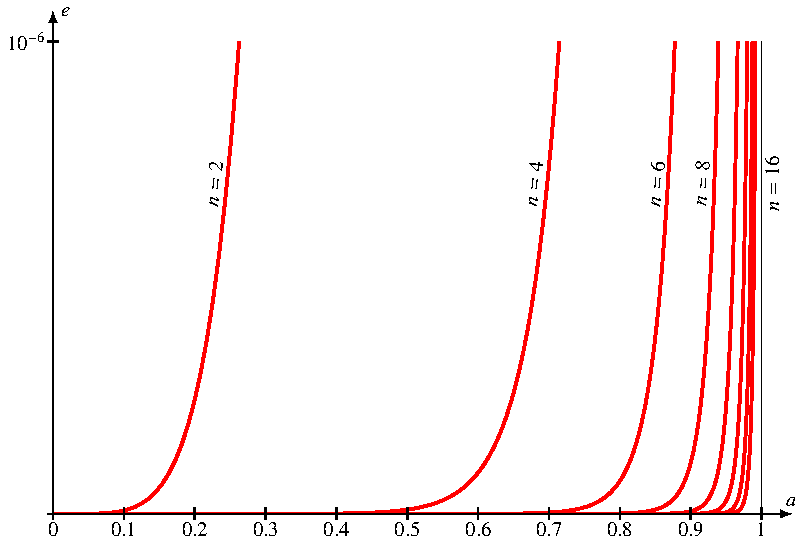
\includegraphics{chapters/060-integral/gq/gq.pdf}
\caption{Approximationsfehler des
Integrals~\eqref{buch:integral:gaussquadratur:bspintegral}
in Abhängigkeit von $a$.
Die Divergenz der Ableitung des Integranden an den Intervallenden
$\pm 1$ führt zu schlechter Konvergenz des Verfahrens, wenn $a$
nahe an $1$ ist.
\label{buch:integral:gaussquadratur:fehler}}
\end{figure}

Zur Illustration der Genauigkeit der Gauss-Quadratur berechnen wir
das Integral
\begin{equation}
\int_{-a}^a \sqrt{1-x^2}\,dx
=
\arcsin a + a \sqrt{1-a^2}
\label{buch:integral:gaussquadratur:bspintegral}
\end{equation}
mit Gauss-Quadratur einerseits und dem Trapezverfahren
andererseits.
Da Gauss-Quadratur mit sehr viel weniger Sützstellen auskommt,
berechnen wir die Trapeznäherung mit zehnmal so vielen Stützstelln.
In den Tabellen~\ref{buch:integral:gaussquadratur:table0.5}
und
\ref{buch:integral:gaussquadratur:table0.999}
sind die Resultate zusammengestellt.
Für $a =\frac12$ zeigt
Tabelle~\ref{buch:integral:gaussquadratur:table0.5}
die sehr schnelle Konvergenz der Gauss-Quadratur, schon mit
12 Stützstellen wird Maschinengenauigkeit erreicht.
Das Trapezverfahren dagegen erreicht auch mit 200 Stützstellen nur
4 korrekte Nachkommastellen.

An den Stellen $x=\pm 1$ divergiert die Ableitung des Integranden
des Integrals \eqref{buch:integral:gaussquadratur:bspintegral}.
Da grösste und kleinste Stützstelle der Gauss-Quadratur immer
deutlich vom Rand des Intervalls entfernt ist, kann das Verfahren
diese ``schwierigen'' Stellen nicht erkennen.
Tabelle~\ref{buch:integral:gaussquadratur:table0.999} zeigt, wie
die Konvergenz des Verfahrens in diesem Fall sehr viel schlechter ist.
Dies zeigt auch der Graph in
Abbildung~\ref{buch:integral:gaussquadratur:fehler}.

\subsection{Skalarprodukte mit Gewichtsfunktion}
Die Nullstellen der Legendre-Polynome ergaben ein gutes
Integrationsverfahren für Polynome auf einem beschränkten
Intervall.
Die Beispiele haben aber auch gezeigt, dass Stellen, wo die
Ableitung des Integranden divergiert, die Genauigkeit stark
beeinträchtigen können.
Ausserdem ist das Verfahren nicht anwendbar auf uneigentliche
Integrale.

\subsubsection{Umgang mit Singularitäten}
Die Lösung des Problems mit Stellen mit divergenter Ableitung
besteht darin, die Stützstellen in der Nähe dieser Stellen
zu konzentrieren.
Die Verwendung einer Gewichtsfunktion $w(x)$ kann genau dies
erreichen.
Statt das Integral einer Funktion $f(x)$ zu bestimmen, 
kann man $f(x)=g(x)w(x)$ schreiben, wobei $w(x)$ so
gewählt werden soll, dass das Verhalten der Steigung an
den Intervallenden gut wiedergibt.
Dies ist mit einer Jacobischen Gewichtsfunktion immer möglich.
Statt der Nullstellen der Legendre-Polynome sind dann die
Nullstellen der Jacobi-Polynome  und die Funktionswete von $g(x)$
an diesen Stellen zu verwenden,  die Gewichte sind
die Integrale von $l_i(x) P^{(\alpha,\beta)}(x)$.

\subsubsection{Uneigentliche Integrale}
Die Berechnung eines uneigentlichen Integrals auf dem Intervall
$(0,\infty)$ oder $(-\infty,\infty)$ ist aus mehreren Gründen nicht
direkt mit dem früher beschriebenen Gauss-Quadraturverfahren
möglich.

Die Stützstellen, die bei der Gauss-Quadratur in einem Intervall
$(a,b)$ verwendet werden, entstehen dadurch, dass man die Nullstellen
der Legendre-Polynome in $(-1,1)$ auf das Intervall $(a,b)$
skaliert.
Dies führt offensichtlich nicht zum Erfolg, wenn ein oder beide
Intervallgrenzen unendlich sind.
Dieses Problem kann dadurch gelöst werden, dass man das unendliche
Intervall $(a,\infty)$ mit
\[
x =  a + \frac{1-t}{t}
\]
auf das Intervall $[0,1]$ transformiert.

Will man beim Intervall $(0,\infty)$ bleiben, dann ist zu beachten,
dass das Integral eines Polynomes immer divergent ist, es ist also
auf jeden Fall nötig, den Integranden durch Funktionen zu approximieren,
die genügend schnell gegen $0$ gehen.
Polynome beliebigen Grades können verwendet werden, wenn sie mit
einer Funktion multipliziert werden, die schneller als jedes Polynom
gegen $0$ geht, so dass das Integral immer noch konvergiert.
Die Funktionen $e^{-x}$ für das Intervall $(0,\infty)$ oder
$e^{-x^2}$ für das Intervall $(-\infty,\infty)$ kommen dafür in Frage.

Um das Integral von $f(x)$ im Intervall $(0,\infty)$ zu berechnen,
schreibt man daher zunächst
\[
\int_0^\infty f(x)\,dx
=
\int_0^\infty g(x)e^{-x}\,dx
=
\int_0^\infty g(x) w(x)\,dx
\quad\text{mit}\quad
w(x)=e^{-x}
\text{ und }
g(x)=f(x)e^x.
\]
Dann approximiert $g(x)$ man durch ein Interpolationspolynom,
so wie man das bei der Gauss-Quadratur gemacht hat.
Als Stützstellen müssen dazu die Nullstellen der Laguerre-Polynome
verwendet werden.
Als Gewichte $w_i$ sind die Integrale der $l_i(x)e^{-x}$
zu verwenden.







\section*{Übungsaufgabe}
\rhead{Übungsaufgaben}
\aufgabetoplevel{chapters/070-orthogonalitaet/uebungsaufgaben}
\begin{uebungsaufgaben}
\uebungsaufgabe{701}
%\uebungsaufgabe{1}
\end{uebungsaufgaben}

